\NeedsTeXFormat{LaTeX2e}
%thesis document class
\documentclass[12pt,twoside,a4paper]{report}

%_________________________________preamble________________________________________

%http://www.howtotex.com/packages/9-essential-latex-packages-everyone-should-use/

%https://www.ctan.org/pkg/nag
\RequirePackage[l2tabu, orthodox]{nag}
%
\usepackage[utf8]{inputenc}

%https://www.ctan.org/pkg/indentfirst?lang=en
\usepackage{indentfirst}

%https://www.ctan.org/pkg/microtype
\usepackage{microtype}

%https://www.ctan.org/pkg/setspace?lang=en
\usepackage{setspace}

%https://www.ctan.org/pkg/amsmath
\usepackage{amsmath, amssymb, amsthm}

%https://www.ctan.org/pkg/siunitx
\usepackage{siunitx}

%https://www.ctan.org/pkg/geometry
\usepackage[a4paper]{geometry}

%https://www.ctan.org/pkg/fancybox
\usepackage{fancybox}

%https://www.ctan.org/pkg/listings
\usepackage{listings}

\lstset{ %
  backgroundcolor=\color{white},   % choose the background color
  basicstyle=\footnotesize,        % size of fonts used for the code
  breaklines=true,                 % automatic line breaking only at whitespace
  captionpos=b,                    % sets the caption-position to bottom
  commentstyle=\color{mygreen},    % comment style
  escapeinside={\%*}{*)},          % if you want to add LaTeX within your code
  keywordstyle=\color{blue},       % keyword style
  stringstyle=\color{mymauve},     % string literal style
}

\usepackage{color}
 
\definecolor{codegreen}{rgb}{0,0.6,0}
\definecolor{codegray}{rgb}{0.5,0.5,0.5}
\definecolor{codepurple}{rgb}{0.58,0,0.82}
\definecolor{backcolour}{rgb}{0.95,0.95,0.92}

\lstdefinestyle{mystyle}{
    backgroundcolor=\color{backcolour},   
    commentstyle=\color{codegreen},
    keywordstyle=\color{magenta},
    numberstyle=\tiny\color{codegray},
    stringstyle=\color{codepurple},
    basicstyle=\footnotesize,
    breakatwhitespace=false,         
    breaklines=true,                 
    captionpos=b,                    
    keepspaces=true,                 
    numbers=left,                    
    numbersep=5pt,                  
    showspaces=false,                
    showstringspaces=false,
    showtabs=false,                  
    tabsize=2
}
 
\lstset{style=mystyle}

%https://www.ctan.org/pkg/url?lang=en
\usepackage{url}

%https://www.ctan.org/pkg/graphicx?lang=en
\usepackage{graphicx}

%https://www.ctan.org/pkg/array?lang=en
\usepackage{array}

%https://www.ctan.org/pkg/fancyhdr?lang=en
\usepackage{fancyhdr}

%https://www.ctan.org/pkg/booktabs
\usepackage{booktabs}

%http://www.tug.dk/FontCatalogue/lmodern/
\usepackage{lmodern}
\usepackage[T1]{fontenc}

%https://www.ctan.org/pkg/hyperref?lang=en
\usepackage{hyperref}
% pdf settings assures outlines being created
\hypersetup{
	pdftitle={Play With Scala},
    pdfauthor={Martin Zuber},
    pdfsubject={Functional Programming in Scala},
    pdfkeywords={functional programming, scala},
    bookmarksnumbered=true,     
    bookmarksopen=true,         
    bookmarksopenlevel=1,       
    colorlinks=true,            
    pdfstartview=Fit,           
    pdfpagemode=UseOutlines,
    pdfpagelayout=TwoPageRight
}

%https://www.ctan.org/pkg/cleveref
\usepackage{cleveref}

\graphicspath{ {figures/} }

%paragraph formatting from thesis guidelines
\setlength{\textheight}{9in}
\setlength{\textwidth}{6in}
\setlength{\oddsidemargin}{.25in}
\setlength{\topmargin}{-.5in}
\setlength{\parindent}{2em}
\setlength{\parskip}{1em}
\setstretch{1.6667}
\hyphenation{itself}

\pagestyle{fancy}
\fancyhf{}
\rhead{Martin Zuber}
\lhead{BSc in Computing}
\cfoot{Page \thepage}

%__________________________________content_____________________________________

\title{Play with Scala\\Functional Programming Course}
\author{Martin Zuber, B00066378 \\ Project Supervisor:  Luke Raeside}
\date{\today}

\begin{document}

\pagenumbering{roman}
\maketitle
\newpage








%_______________________________chapter_______________________________________
\chapter*{Declaration}
I hereby certify that this material, which I now submit for assessment on the programme of study leading to the award of Degree of Honours B.Sc. in Computer Science in the Institute of Technology Blanchardstown, is entirely my own work except where otherwise stated, and has not been submitted for assessment for an academic purpose at this or any other academic institution other than in partial fulfilment of the requirements of that stated above.









%_______________________________chapter_______________________________________
\chapter*{Acknowledgements}
In performing my assignment, I had to take the help and guideline of some respected persons, who deserve my greatest gratitude. The completion of this assignment gives me much Pleasure. I would like to show my gratitude to the project supervisor Dr Luke Raeside, Institute of Technology, Blanchardstown for giving me good guidelines for the thesis throughout numerous consultations. I would also like to expand my deepest gratitude to all those who have directly and indirectly guided me in writing this thesis, especially Dr Markus Hofmann.








%_______________________________chapter_______________________________________
\chapter*{Abstract}
This paper is dedicated to computer programming with the focus on programming styles found in modern application development. The idea for the project came to life when I, the author and computer science student realized there are programming styles other than imperative object-oriented programming. Namely functionalk programming paradigm. The lack of a study material dedicated to the functional programming withing the ITB Computer Science course curriculum and my curiosity toward the subject I decided to research and to learn the paradigm.

This paper is discussing functional programming paradigm with Scala programming language and web application development process using Play! Framework. The target audience is any computer science student with intermediate knowledge of a programming language such as Java and with an understanding of some of the object-oriented programming principles such as inheritance and polymorphisms.

Please keep in mind that I had no knowledge of a functional programming, Scala programming language or Play Framework prior to this endeavour. This document is basically a report of a student learning basics of these concepts and tools. I can only hope that I would be able to communicate clearly what I learn and I sincerely hope this document would be useful to someone.

\listoffigures
%\listoftables
\tableofcontents{}
\pagenumbering{arabic}











%_______________________________chapter_______________________________________
\chapter{Introduction}\label{1}

%____________________________section____________________________
\section{Introduction}\label{1.1}
In the current world of multi-core processor computers, distributed systems and big data, we are witnessing a paradigm shift in the computational model used in application development industry. It is the shift from imperative programming style toward declarative programming and the rise of the functional programming languages\cite{1}. JVM ecosystem is no exception.

Even though Java being still most used JVM language, some other languages such as Scala, Groovy and Clojure are getting more popular every day. There are various reasons for the popularity where each language has its own strengths, but what they all have in common is a much richer support for functional programming in comparison to Java. Java itself with recent SE 8 update adapted to this trend and brought limited support for functional programming as well.

Scala programming language \cite{2} is getting a big momentum over the last few years in the industry\cite{3}. Companies such as Twitter, LinkedIn\cite{4}, Netflix, Sony, Foursquare had switched to Scala in their application development. Scala is being a big player in the realms of Reactive programming, Distributed Systems and Big Data\cite{5}.

\subsection{Some of the reasons for Scala success}\label{1.1.1}
\begin{itemize}\itemsep1pt \parskip0pt \parsep0pt
\item Scala is an expressive but elegant multi-paradigm programming language with the performance comparable to Java. It is often regarded as \emph{"the most evolved programming language on the planet"}. Scala has better support for object-oriented programming than Java (better object model, higher-kinded parametric polymorphism, multiple inheritance, built-in singleton pattern and more. At the same time, Scala has advanced support for functional programming comparable to ML-like languages, such as Haskell, F\# or oCaml. In this context, Scala emphasizes immutability by default, supports first-class and higher-order functions, lambdas, currying and partial function applications, built-in lazy sequences, monads, algebraic data structures, type classes, pattern matching, for comprehension and more.
\item Scala compiles to JVM byte code.class files which mean that language is fully compatible with existing Java libraries and frameworks and vice versa. Mixed Java / Scala projects are quite common with Scala compiler support for cyclic compilations. Many projects written in Java were refactored to Scala to utilize the language expressiveness or features which are just missing in Java, such as Scala \emph{Actors} concurrency model.
\item Scala is \emph{scalable} by design, with a powerful compiler supporting plug-ins and advanced macros. The compiler is written in Scala itself and both, the language and the compiler are open source projects. Scala supports operator overloading and being a functional programming language, it is a well suited for the development of interpreters and Domain Specific Languages (DSL).
\item The existence of powerful, open source and award-winning frameworks\cite{6}, toolkits, and platforms written in Scala, such as Akka, Spark, Play\cite{7} is a powerful drive for language adoption in enterprise development.
\end{itemize}

%____________________________section____________________________
\section{Aims and Objectives}\label{1.2}
The aim of this project is to study Scala programming language, functional programming paradigm and to develop a learning material in the form of lecture prototypes for a fictional "functional programming" college module. The idea came to life in the moment I saw that there is no module dedicated to functional programming in the final year of my studies in ITB. Effectively I realized that functional programming was not mentioned once in any of the modules throughout all four years of Computer Science course.

The secondary aim of the project is to deliver the lectures to potential students who are also interested in functional programming in the form of simple web application. The application will be developed using Play Framework rapid web development platform. In this endeavour, I will concentrate on studying the framework, rather than to dedicate too much valuable time to web application development. I have developed a number of web pages, web APIs and Single Page Applications (SPA) during my studies here in ITB. On the other hand, I did not have a chance to learn any enterprise web development platform other than JavaEE.

\subsubsection{Reasons:}

\begin{itemize}\itemsep1pt \parskip0pt \parsep0pt
\item Strong personal interest in functional programming.
\item Lack of modules dedicated to functional programming in ITB curriculum.
\item Solid background in JVM platform.
\item Desire to pursue a professional career in Java / Scala development.
\item Interest in Lightbend Reactive Platform\cite{32} (Play Framework).
\end{itemize}

\subsection{Proposed functionality of the web application}\label{1.2.1}
\begin{itemize}\itemsep1pt \parskip0pt \parsep0pt
\item A student can register the account.
\item The authenticated student will gain access to the functional programming with Scala lectures and exercises.
\item The student can adjust the account settings.
\item The student will have access to an online Scala interpreter where he could carry out coding exercises.
\item The student will be able to communicate with other users through a chat window or other messaging functionality.
\end{itemize}

%____________________________section____________________________
\section{Main Research Questions}\label{1.3}
\begin{itemize}\itemsep1pt \parskip0pt \parsep0pt
\item What exactly is functional programming and what benefits does it bring to application development?
\item What is Scala programming language and how it supports the functional programming?
\item How would I explain functional programming to others?
\item What exactly is Play Framework and how can I develop a web application with it?
\item What are the advantages and disadvantages of the Play Framework in terms of productivity, performance and scalability and in comparison to other frameworks?
\end{itemize}

%____________________________section____________________________
\section{Justifications / Benefits}\label{1.4}
As mentioned earlier, the functional programming is totally ignored by ITB Computer Science course curriculum. In my opinion, this creates an 'educational gap' in the curriculum. Personally, I feel that the topic belongs in the course and it is the natural progression from imperative object-oriented programming and design patterns which had strong coverage in the third year of the course.

\textbullet \textbf{ Filling the 'educational gap' in the Computer Science course curriculum by creating learning web resource.}

The preliminary research on the current state of the application development industry is suggesting that fluency in a functional programming language is a really valuable skill for any developer to possess. Developers able to code using languages such as Scala, Clojure, F\# or Lisp dialects are in high demand. Reasoning about the functional programs requires different ‘mind-set’ or ‘thought process’ in comparison with object-oriented programming. Even if one would never use purely functional programming professionally, understanding of the concepts will make one a better programmer overall.

\textbullet \textbf{ Acquiring valuable skills and deeper insides into different programming paradigms and design patterns.}

Also, Scala seems to be very elegant language and takes the good design ideas from many other programming languages. The language was designed with the scalability of the syntax taken in the consideration, which allows the language to 'shape-shift' towards the needs of its users. In my opinion, the Scala programming language would be the right tool for me to learn functional programming paradigm. In my preliminary research I found number of books dedicated to functional programming with Scala.

\textbullet \textbf{ Learning Scala programming language and Java Virtual Machine (JVM).}

Even though learning functional programming with Scala is the main aim of this project, the additional work will be carried out by exploring Play Framework and developing a web application. The preliminary research suggests the framework is a powerful tool for rapid web development. Play seems to be heavily inspired by Ruby on Rails. It supports reactive web application development and seems to be a cleaner alternative to legacy Java Enterprise stack \cite{8}.

\textbullet \textbf{ Building valuable skill set in contemporary web application development.}

%____________________________section____________________________
\section{Feasibility}\label{1.5}
\textbf{Project requirements}
\begin{itemize}\itemsep1pt \parskip0pt \parsep0pt
\item Access to relevant study material and tutorials dedicated to Scala programming language and Play. There is no material available in ITB library, but there is a number of books published and available over the internet. \textit{Estimated cost is 100 euros.}
\item Access to personal computer. I'm the owner of the laptop computer, which should serve as the project workstation without too many constraints. Additional research must be done to decide on the operating system and other tools. Using free software is most desired.\textit{Estimated cost is 0 euros.}
\item Access to the internet, deployment, DNS and versioning control services, printer and thesis binding.\textit{ Estimated cost is 300 euro.}
\item At least 10 hours per week to carry out the project related work for the whole project duration. This estimation is based on personal experience I gained by working on two academic projects during my studies and on experience working on a research project as part of the summer internship.
\end{itemize}
In my opinion, all the requirements could be met to assure this project feasibility with the minimal cost associated. With proper planning, use of the personal assets and free software when possible, I should be able to meet the project goals within the given time scale.

%____________________________section____________________________
\section{Proposed Methodologies}\label{1.6}

\subsection{Literature Review}\label{1.6.1}
The first step is to carry out the research on functional programming \cite{9}, Scala programming language \cite{10}, MVC design pattern and Play Framework \cite{11}. I'm planning to use dedicated books I acquired recently, plus online tutorials and blogs. I will analyze, summarize, and carry out the coding tutorials. The thorough literature review at the beginning should lay a foundation for following web application development. I will continue to research relevant materials for the whole duration of the project.

\subsection{The Web Application Development}\label{1.6.2}
The real challenge lies in the fact that I have a little experience developing web applications using MVC framework and no skills in technologies I decided to use during this project. I have only general ideas how to design such an application. Only layers I can design reasonably well in advance are the database relations and user interface.\par
Therefore, I must approach this problem using some kind of adaptive methodology and avoid 'a big design in advance' approach. I would argue that Prototyping SDLC is the best methodology to carry out the development. In this model, the developer basically re-analyzes, re-designs, re-implements and re-test application prototype until the product is accepted by the client.
\begin{figure}[!ht]
	\centering
		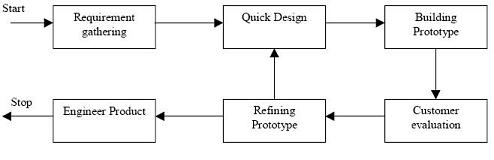
\includegraphics[width=0.8\textwidth, totalheight=5.5cm]{prototyping}
	\caption{\textit{Prototyping SDLC diagram}}
	\label{f1.1}
\end{figure}
Instead of creating 'a big design in advance', prototyping methodology is allowing the developer to change the design with each iteration of the design / development / evaluation / refining circle. I should expect major changes in design based on my lack of experience in web development and technologies I decided to use. The prototyping methodology will allow me to have a simple, but functioning prototype reasonably early. As more insights are acquired from the research, the prototype can be re-designed to implement additional functionality or re-evaluate the design.

%____________________________section____________________________
\section{Project Plan}\label{1.7}
\textbf{Work Breakdown Structure (WBS)}
\begin{enumerate}\itemsep1pt \parskip0pt \parsep0pt
\item \textbf{Research.}
	\begin{enumerate}\itemsep1pt \parskip0pt \parsep0pt
	\item Research on Scala programming language design ideas and syntax, MVC design pattern, Play framework, user interface and database design.
	\item Literature Review of papers dedicated to the functional programming paradigm and test driven rapid web application development with Play.
	\item Building development platform.
	\end{enumerate}
\item \textbf{Front-End design.}
	\begin{enumerate}\itemsep1pt \parskip0pt \parsep0pt
	\item Creating wire-frame design for new view.
	\item Constructing the view.
	\end{enumerate}
\item \textbf{Database Design.}
	\begin{enumerate}\itemsep1pt \parskip0pt \parsep0pt
	\item Adding the database entity for new view.
	\item Designing the relationships with existing entities.
	\end{enumerate}
\item \textbf{Prototype Development.}
	\begin{enumerate}\itemsep1pt \parskip0pt \parsep0pt
	\item Creating the controller object.
	\item Creating unit tests.
	\item Implementing method bodies using test driven development methodology.
	\item Repeating the steps 1, 2, 3 with additional functionality until the final product is build.
	\end{enumerate}
\item \textbf{Quality Assurance.}
	\begin{enumerate}\itemsep1pt \parskip0pt \parsep0pt
	\item Performing integration tests of the whole MVC pipeline.
	\item Performing user tests.
	\end{enumerate}
\item \textbf{Post Implementation Maintenance.}
	\begin{enumerate}\itemsep1pt \parskip0pt \parsep0pt
	\item Making prototype production ready and deploying the prototype.
	\item Monitoring deployed application and adding more content.
	\item Adding content to the application.
	\item Working on project Report.
	\item Repeating steps 5.(a), 5.(b), 6.(a), 6.(b), 6.(c), 6.(d)
	\item Report Binding.
	\end{enumerate}
\end{enumerate}
\begin{figure}[!ht]
	\centering
		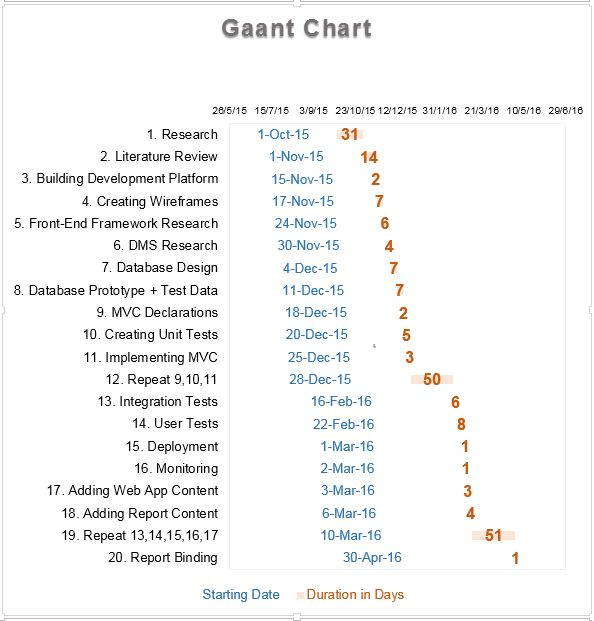
\includegraphics[width=0.9\textwidth,totalheight=9cm]{gaant}
	\caption{\textit{Gaant Chart}}
	\label{f1.2}
\end{figure}

%____________________________section____________________________
\section{Expected Results}\label{1.8}
The project would be considered successful if it would meet at least two following criteria and goals. In the case of three or more goals accomplished I would consider project outcome to be very successful.
\begin{enumerate}\itemsep1pt \parskip0pt \parsep0pt
\item The gain in Scala coding skills and creation of enough learning material content for Scala course web application.
\item The comprehensive research on the functional programming paradigm and design patterns performed and gained the ability to code in the declarative style.
\item The delivery of fully functioning prototype of Scala course learning web application.
\item The acquisition of skill-set in rapid web development using Play framework.
\end{enumerate}

%____________________________section____________________________
\section{Conclusion}\label{1.9}
At the end of this project, I will hopefully introduce some of Scala dedicated learning material in the form of an interactive web application. It can be used in a fictional course module for a fictional college. The application main purpose is to promote the interest in Scala programming language and functional programming paradigm. Especially on the personal level. After three years of my studies with ITB, I didn't learn anything about functional programming. I chose this project so I can gain a knowledge and skills which are really missing in my skill-set and which could prove very useful in the future. I hope as a fourth year student I am ready to face this challenge.\par
This research project will not contribute at all to the discipline area. Maybe only in a sense that it will hopefully bring one more student with the passion for programming languages to the functional programming paradigm. And maybe if other students or lecturers will see how elegant and declarative functional programming really is, the contribution could be a bit more significant.











%_______________________________chapter_______________________________________
\chapter{Literature Review}\label{2}

%____________________________section____________________________
\section{Introduction}\label{2.1}
Computer programming is a fascinating and vast subject to study. Programming languages began as an attempt to translate the human language and the way of human thinking into the language of a computer.\par
The idea was to make it easier, more efficient for programmers to write the programs. With the evolution of computers, as the problems to solve became more complex, the programs became larger and more sophisticated. The programming languages quickly evolved into the forms commonly referred to as high-level programming languages. In these forms, the programming languages are hiding the internal hardware details and offer a higher level of abstractions allowing programmers to write the programs using familiar terms with an ability to model real life objects.\par
The purpose of this paper is to review some of the studies dedicated to concepts and design ideas behind the high-level programming languages. The research done in this field is immense. It is out of the scope of this paper to cover every concept,paradigm, or language and rather study some of the most important concepts in general. Then I will continue to study research papers dedicated to two most popular paradigms - object-oriented and functional programming. I will try to identify and discuss their key concepts, strength, and weaknesses and outline their history in short. I chose reading materials with a secondary intention to lay down a foundation for further studies toward a deeper understanding of the paradigms and transitions between them.

%____________________________section____________________________
\section{General Concepts}\label{2.2}
In \emph{The Conception, Evolution, and Application of Functional Programming Languages}\cite{12} author defined a programming paradigm as an approach to a computer programming based on a coherent set of principles or a mathematical theory. The purpose for a paradigm existence is to solve a specific type of a problem. Each paradigm consists of a number of concepts. Any programming language can support one or more paradigms and the language which support more than one paradigm is called the multi-paradigm programming language. Different languages can interpret the concepts of a paradigm differently and often the implementations differ from language to language as well. The author listed around 30 useful programming paradigms implemented by modern programming languages.

Author then identified the two most important properties which differentiate the programming paradigms:

\begin{enumerate}\itemsep1pt \parskip0pt \parsep0pt
\item \textit{Observable nondeterminism} is when a program is not completely determined by its specification. In other words with each execution the same program can produce different results. Observable nondeterminism is caused by the run-time scheduler and its usual effect is a race condition, which is often used as the synonym for Observable nondeterminism.
\item \textit{Named state} is an ability of a program to store values in time. This ability is highly influenced by the paradigm it contains it.
\end{enumerate}
\begin{figure}[!hb]
	\centering
		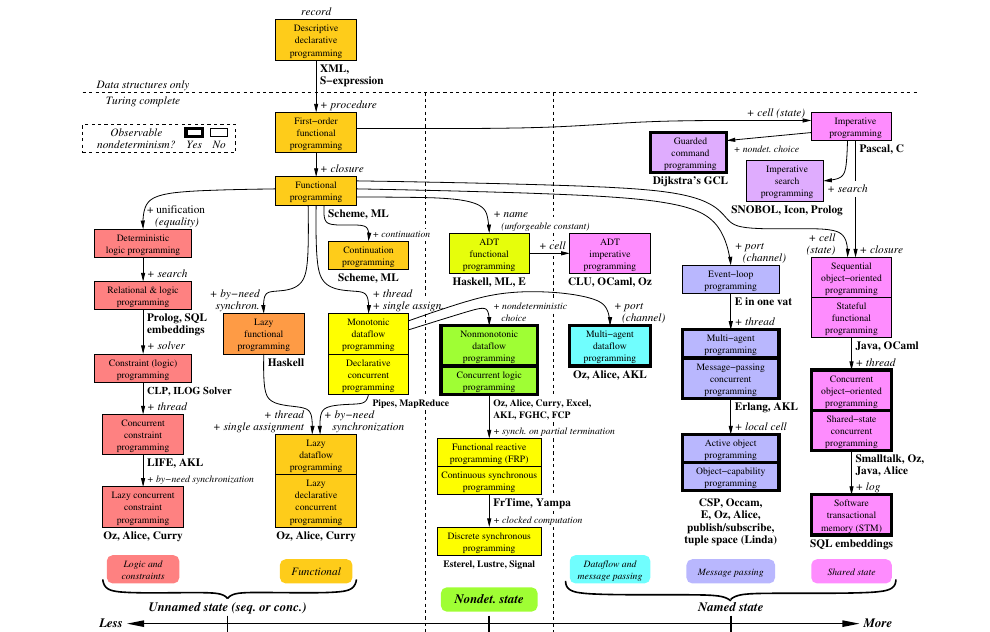
\includegraphics[width=1\textwidth,totalheight=12cm]{taxonomyDiagram}
	\caption{\textit{Taxonomy of programming paradigms (Van Roy, page 15)}}
	\label{f2.1}
\end{figure}

As mentioned before, the programming paradigms are based on a number of concepts. Author identified four most important programming concepts:
\begin{enumerate}\itemsep1pt \parskip0pt \parsep0pt
\item \textbf{Record} is a data-structure. Every programming language should be able to work with records. Arrays, lists, strings, trees and hash tables are derived from records.
\item \textbf{Lexically scoped closure} is a record storing a function together with an environment referenced at the time of that function definition. Closure is a very powerful concept and constructs such as \textit{objects} or \textit{control structures} have been implemented with closures in many programming languages.
\item \textbf{Independence} is when a program is constructed from independent parts. When parts don’t interact with each other we call them \textit{concurrent}. When an order of the execution is given, the parts are called sequential. The interaction between the parts is called communication. Author recognizes three levels of concurrency:
    \begin{enumerate}\itemsep1pt \parskip0pt \parsep0pt
    \item \textit{Distributed system,} where concurrent activities (parts) are computers.
    \item \textit{Operating system,} where concurrent activities are processes. This level of concurrency is often called competitive concurrency because the processes are competing for access to system resources.
    \item \textit{Inter Process,} where concurrent activities are threads. This level of concurrency is called \textit{cooperative concurrency} because the threads are cooperating to achieve the result of the process. There are two popular paradigms for inter process concurrency: \textit{Shared state concurrency}, where shared data are accessed by threads using control structures called \textit{monitors}. The second approach is \textit{message-passing concurrency}, where threads are communicating by sending messages to each other.
    \end{enumerate}
\item \textbf{Named State} Author showed how named state could be implemented with a help of internal memory (variables).
\end{enumerate}

%____________________________section____________________________
\section{Specific Characteristics}\label{2.3}

\subsection{Object Oriented Programming}\label{2.3.1}
In \emph{A Survey of Object Oriented Programming Languages}\cite{13} authors argued that consensus on what key concepts of Object Oriented Programming still don't exist. They argue that the most fundamental concepts behind the paradigm are as follows:
\begin{enumerate}\itemsep1pt \parskip0pt \parsep0pt
\item \textbf{Class} is a mechanism which group together attributes and methods with common properties. The class describes the run-time behavior of the objects instantiated from it. The well-designed class would have an immutable interface clients can use.
\item \textbf{Abstraction} is a simplified view of reality. Presented to clients by class methods and attributes.
\item \textbf{Inheritance} is a mechanism to create hierarchical class designs by creating a child class of the original class. A child class inherits the parent class behavior which can be then extended. Multiple inheritance allows for a class to inherit the behavior of multiple parent classes.
\item \textbf{Encapsulation} is hiding implementation details within the class. Only the interface is presented to the
clients.
\item \textbf{Polymorphism} is allowing to similar looking structures to handle a variety of objects.
\end{enumerate}
Authors then discussed inheritance and polymorphism in detail. I will outline the important key points.

\subsubsection{Inheritance}
As mentioned earlier the inheritance brings the hierarchical relationship into the class model. Authors pointed out that many languages define the most generic class that is an ancestor for all the classes in the language. This applies that any class can be downcast to the pointer of that ancestor. Authors pointed out that inheritance provides the ability to represent an \textit{“is a”} relationship in software. This relationship can be violated if child class extends the inherited code the way which changes the code semantics. It is the reason for the inheritance to be used with caution.

Inheritance also allows to represent generalization /specialization relationships with method redefinition. This functionality is breaking the encapsulation because the child class has access to parent class hidden methods and attributes. This problem can be addressed by defining a well-defined interface for the descendants. Authors argued that literary every object-oriented language provides the ability for a child class to invoke parent class methods. Even those methods which were redefined in the child class.

Some of the languages support the feature which restrict method redefinition. A method is marked \textit{‘frozen’} or \textit{‘final’} and no child class can redefine this method. Authors warned that inheritance has also an adverse effect on synchronization requirements of a concurrent object. This problem is usually named \textit{‘inheritance anomaly’}. The problem arises when a class with concurrent code is derived. The careful redefinition of the inherited methods is necessitated to preserve the synchronization requirements. This necessity denies \textit{‘reuse’} benefits of inheritance. The multiple inheritance potential risks were then discussed in details. Authors explained various problems which could arise such as directed acyclic graph in a class hierarchy, method name collisions or repeated inheritance problem.\par
Authors outlined various solutions to deal with the problems and outlined the alternatives to multiple inheritance used by some of the object-oriented programming languages such as interfaces, mixins or delegation.

\subsubsection{Polymorphism}
As mentioned earlier, polymorphism allows programmers to write functions and classes which work uniformly with different types. Authors listed four distinct types of polymorphisms grouped into two categories. \textit{Ad-hoc Polymorphism} and \textit{Universal Polymorphism.} The difference between the categories is based on the fact that ad-hoc polymorphic functions execute code only for a small set of potentially unrelated types while universal polymorphic functions execute the same code for an infinite number of types.

Authors then defined the two types of ad-hoc polymorphism: The first type is \textit{Overloading Polymorphism}, where the polymorphic function has the same name, but a different signature. Within this type authors distinguished between a \textit{method} overloading and \textit{operator} overloading and discussed each in detail.\par
The second type of ad-hoc polymorphism is \textit{Coercion Polymorphism}. With coercion, the value of an argument can be converted to the value of another argument from the list of a method arguments. Authors pointed out that the difference between those two of ad-hoc polymorphism types is often blurry, especially in untyped and interpreted programming languages. The universal polymorphism is divided to two kinds as well. The first kind is \textit{Parametric Polymorphism} aka generic programming. Generic programming uses type parameters to determine the type of a method argument. Authors pointed out that parametric polymorphism is only relevant for statically typed languages because dynamically typed languages infer types at run-time and hence have generic programming built into them. The second kind is \textit{Inclusion Polymorphism}, which gives different classes the ability to handle the same functionality.

Inclusion Polymorphism is what we call \textit{Inheritance} in object oriented programming. Inclusion polymorphism is implemented through \textit{dynamic binding} or sometimes called \textit{late binding} because a method is bind to the message at the run-time. It is relevant for situations when a child class has an overridden method of the parent class and it is not obvious which method is being invoked. The search for the right method is then performed by the compiler (interpreter) at run-time. The dynamic binding uses the most specific version of a method.\par
Authors mentioned that some of the languages implement static binding where methods are bind to messages at compile time and it will always bind to a base class method version.

\subsection{Functional Programming}\label{2.3.2}
In \textit{The Conception, Evolution, and Application of Functional Programming Languages}\cite{12} the author distinguished four key characteristics of modern functional programming languages.

\subsubsection{Higher-Order Functions}
In functional programming, the functions are treated as \textit{'first class values'}, which means that they can be stored in data structures, passed as other function arguments and returned as results. The author pointed out that the function is the primary abstraction mechanism over values. He showed with examples how to compose higher-order functions.

\subsubsection{Lazy Evaluation}
Often called Non-Strict Semantics or call-by-need. Its primary feature is that arguments in a function call are evaluated at most once. In some cases, it does no evaluation at all. The author
explained with the help of an example how lazy evaluation frees a programmer from concerns about evaluation order and pointed out the ability of the lazy evaluation to compute with infinite
data-structures.

\subsubsection{Data Abstraction Mechanisms}
The author pointed out that a data abstraction improves modularity, security and clarity of programs. He explained that modularity is improved because one can abstract away from
implementation. Data abstractions prohibit interface violations which improves security and that programs are clearer because of the self-documenting quality of the data abstractions. He argues
that \textit{strong static} typing eliminates type violations and run-time errors. He continued the discussion by describing \textit{algebraic} (concrete) data types, \textit{type synonyms}, and \textit{abstract data types}.

\subsubsection{Pattern Matching}
The lack of side-effects in functional programs allows to apply pattern matching or sometimes called equational reasoning. The author explained the basics behind the feature with the help of code examples and outlined some of pattern matching shortcomings.\par
In \emph{Why Functional Programming Matters}\cite{14} author summarizes functional programming characteristics and advantages as they are usually used in the literature as follows:
\begin{itemize}\itemsep1pt \parskip0pt \parsep0pt
\item The functional program consists of functions.
\item The functional program uses no mutable variables which, in general guarantee that program contains no side-effects. A program without side-effect is free of a major source of bugs.
\item Since a function call produces no side-effects and for given arguments produces the same calculation result independently on when it is evaluated, the order of execution is irrelevant and functional programs are referentially transparent. This freedom makes functional programs easier to reason about.
\end{itemize}

The author argues that this often used list of strengths of functional programs is describing what functional programming is not (no assignments, no side-effects, no flow of control) and fails to emphasize what functional programming actually is. The list fails to emphasize the modularity as probably the most powerful characteristic and advantage of functional programs. He convincingly argues the ability of higher-order functions and lazy evaluation to increase the modularity by serving as a ‘glue’ for the program fragments. He provides a number of examples with code to support his claims.

%____________________________section____________________________
\section{Short History}\label{2.4}

First generally accepted object-oriented programming language is Simula (1967). With the introduction of Smalltalk (1962-1980) the paradigm gained some momentum. Most of the concepts of object-oriented programming were implemented in Smalltalk. In early 1980 the concepts were integrated into C programming language and resulting language was called C++. In the 1990s, the similar language was developed called Java by Sun Microsystems. Java became soon one of the most popular object-oriented languages. Then in 2000, Microsoft announced .NET platform and C\# programming language. C\# is in many respects similar to Java. \cite{13}

Functional Programming is heavily influenced by lambda calculus invented by Alonzo Church in 1936. First of the programming languages implementing lambda calculus was Lisp specified in 1958. Next significant language in terms of contributions to functional paradigm was Iswim introduced by Peter Landin in 1966. Probably the first functional language which received wide-spread attention was FP specified in 1978. In mid 70’s several research projects related to functional programming emerged in the UK. Specifically the work of Gordon, Milner, and Wadsworth. They developed ML programming language which brought the invention of the type system (Hindley-Milner Type System). In early 80’s David Turner at the University of Kent developed three languages which most faithfully characterize “modern school” of functional programming: SASL, KRC and Miranda. \cite{12}

In later 1990s and after 2000 the functional programming has gained a great momentum and penetrated mainstream programming. Haskell, F\#, Clojure, Scala are some of the examples of functional programming languages. Many object-oriented languages added functional features and become multi-paradigm languages. Java, Python, C\# are examples of such.

%____________________________section____________________________
\section{Interesting Ideas for Further Study}\label{2.5}

\subsection{A Definitive Programming Language}\label{2.5.1}
In \emph{Programming Paradigms for Dummies: What Every Programmer Should Know}\cite{16} the author is presenting four research projects, each trying to solve a very different problem, but all four project considered language design as a key factor to achieve success. Turned out that programming languages invented in each project have very similar structure supporting same paradigms: strict functional programming, declarative concurrency, asynchronous message passing and global named state. The invented languages are Erlang, E, Distributed Oz and Didactic Oz. One could infer ideas for a design of ‘perfect language’ and it could be quite interesting to study those four programming languages.

\subsection{Artificial Intelligence}\label{2.5.2}
In \cite{14} the author of the paper is using examples of composing programs from lazy evaluated higher-order functions. The final example is the alpha-beta heuristic algorithm. This algorithm is often used in computer games to estimate how good a player position is in the game. The author used Miranda programming language syntax, but it would be very interesting to implement the algorithm in some other functional programming language such as Scala or Haskell.

\subsection{LambdaFicator}\label{2.5.3}
Java 8 update brought a few functional programming features in the language. Namely functions as first class values, lambda expressions and closures. Also fluent Stream API which uses monads, lazy evaluation, and higher-order functions. In \emph{Crossing the Gap from Imperative to Functional, Programming through Refactoring}\cite{15} authors presented the analysis, design, implementation and evaluation of LAMBDAFICATOR, the automatic refactoring tool, which converts old-style code prior to Java 8 update into the functional style. Namely tool does two refactorings:

\begin{itemize}\itemsep1pt \parskip0pt \parsep0pt
\item Anonymous inner classes to lambda expressions
\item External iterators to internal iterators (from \textit{for loops} to Stream API \textit{higher order function chains})
\end{itemize}

In the paper, authors discussed their motivations, outlined the implementation algorithm in the detail and determined the usefulness with a thorough evaluation. They applied the tool to four open source projects (ANTLRWorks, Apache Ivy, Junit, Hadoop) with very successful results. For example, the first type of refactoring reduced the number of source code lines by 2213 with 100 percent accuracy.\par
The tool is open source and available for download and would be very interesting to study it deeper and implement it using some other programming language such as Scala or Haskell.

%____________________________section____________________________
\section{Conclusion}\label{2.6}
The main purpose of this research was to study two most popular programming paradigms: object-oriented and functional programming. To identify and understand the key concepts and to
find the similarities and differences. The first step was to understand general programming concepts such as record, closure, state and concurrency. 

I continued to study characteristics of object-oriented programming languages. I learned that main building blocks of object-oriented programs are classes organized into hierarchies based on inheritance. I learned about polymorphism, the powerful feature of programming languages in general. 

Also, I studied papers dedicated to functional programming and I found out that functional programs are built from functions, which are then composed together to modules and programs. I was shown the elegance of lazy evaluation and pattern matching. I learned that functional programs are trying to eliminate state and to stay referentially transparent.










%_______________________________chapter_______________________________________
\chapter{Analysis and Design}\label{3}

%____________________________section____________________________
\section{Introduction}\label{3.1}
In this section, I will discuss the approach to the content and web application design. The main aim of this project is to explore functional programming methodologies, develop a learning material content dedicated to the functional programming with Scala programming language. The secondary aim is to develop a simple web application which would deliver the learning material to a potential consumer. 

%____________________________section____________________________
\section{Proposed Methodology}\label{3.2}

\subsection{Learning Material}\label{3.2.1}
The lectures will have a form of static text with code examples and coding exercises, The references to cited paragraphs and the source study material will be included. There will be a link to online Scala REPL\cite{18} available in each lecture, offering to a student an environment to test the code examples and carry out the exercises. Lectures are proposed to be short, covering only one concept or a feature at the time. Lectures will be formatted using Markdown. Markdown is a text-to-HTML conversion tool for web writers. Markdown allows you to write using an easy-to-read, easy-to-write plain text format, then convert it to structurally valid XHTML (or HTML)\cite{20}.

Scala is an elegant but complex programming language. I realized that to be able to study functional programming with Scala, the student will need to learn the language syntax first. Even though Scala programs resemble Java programs in many ways and they can seamlessly interact with code written in Java\cite{17}, it doesn't mean that Scala is just Java with slightly different syntax. In contrary, Scala is purely object-oriented, has a different object model, a richer type system with the type inference, supports multi-inheritance through mixins, pattern matching, implicit references, partial function applications, operator overloa and much more. Basically, Scala is much richer language than Java and considered by many to be the most evolved programming language.

The lectures will cover the functional programming paradigm using Scala programming language in proposed form. These lectures will not cover the Scala syntax, but rather how to design functional programs and how to reason about them.

\subsection{Web Application}\label{3.2.2}
Secondary aim of this project is to develop a simple web application which will publish the learning material over the internet to the potential students. Idea is to develop this web application using Scala and functional programming style. This could be quite a challenge, because I must first learn and language and the style, which is actually the main aim of this project. If I fail to grasp the concepts I will be not able to build the application. I chose Play Framework to carry out the implementation of the application because it supports both Java and Scala programming languages and therefore in the case I will feel not comfortable enough to carry out development in Scala I can work in Java.

\begin{figure}[!ht]
	\centering
		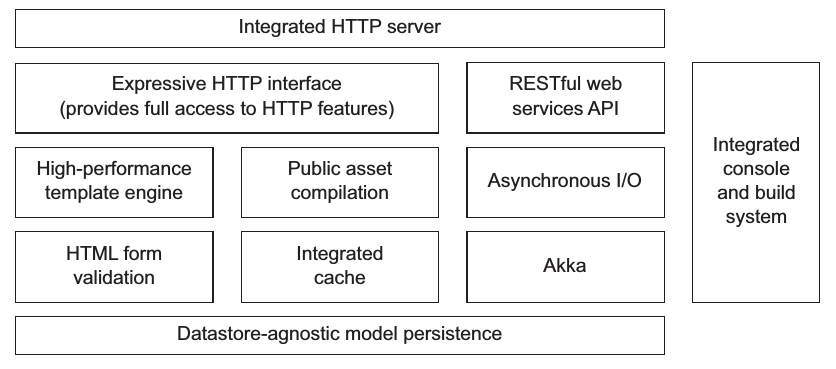
\includegraphics[width=0.9\textwidth, totalheight=8cm]
		{play_stack}
	\caption{\textit{Play Framework Stack}}
	\label{f3.1}
\end{figure}

\textbf{Play Framework Key Features Overview\cite{11}}

\begin{itemize}\itemsep1pt \parskip0pt \parsep0pt
\item Declarative application URL scheme configuration
\item Type-safe mapping from HTTP to Scala API
\item Type-safe templates
\item Embraces HTML5
\item Live code changes when you reload the page in your web browser
\item Full-stack framework (\cref{f3.1}), including persistence, security and internationalization
\end{itemize}

\textbf{Play versus Java EE}

From \cref{f3.2} is apparent how the framework embraces the simplicity in comparison with layered Java Enterprise Edition architecture. Whole framework stack is build on top of Netty\cite{19} client-server framework and doesn't require an application server container. Netty assures high performance of the stack and simple deployment of the application. Play has both, Java and Scala APIs (Application-Programming Interface) which will allow me use functional programming with Scala. I will discuss the framework in more depth in Back End Desing \cref{3.8} and Implementation \cref{4}.
\begin{figure}[!ht]
	\centering
		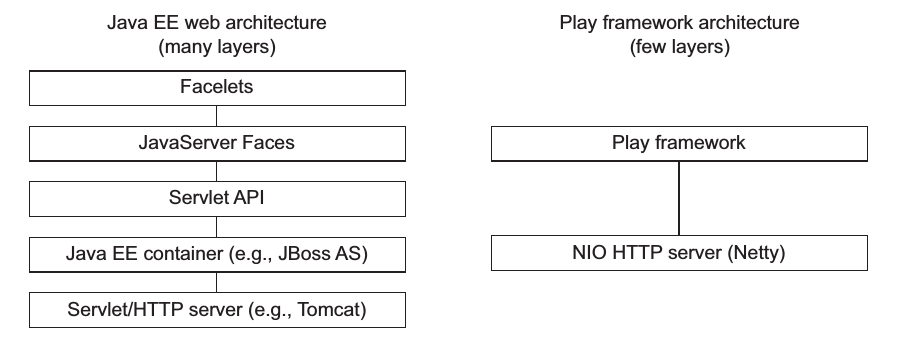
\includegraphics[width=0.9\textwidth, totalheight=8cm]{play_vs_java_ee}
	\caption{\textit{Java EE 'lasagna' architecture versus Play architecture}}
	\label{f3.2}
\end{figure}

\textbf{SDLC - Prototyping Model}\par
As discussed in Proposed Methodologies for The Web Application Development \cref{1.6.2}, I will use Prototyping Software Development Life-Cycle Model to develop the web application. Each step in development cycle is already listed and explained in Work Breakdown Structure \cref{1.7} of Project Plan.

%____________________________section____________________________
\section{Proposed Tools}\label{3.3}

\subsection{Hardware}\label{3.3.1}
The project will be developed on DELL Latitude E5540 laptop machine lent to me by School of Computer Science, UCD where I work part-time as a research assistant. The laptop has following specification and should be sufficient to support this project development.

\begin{itemize}\itemsep1pt \parskip0pt \parsep0pt
\item \textbf{Procesor:} Intel Core i5-4310 CPU 2.00GHz x 4
\item \textbf{Memory:} 8GB RAM
\item \textbf{Graphics:} Intel Haswell Mobile
\item \textbf{Hard Disk:} 463 GB
\end{itemize}

\subsection{Software}\label{3.3.2}
I decided to use an open source, or at least free software tools. The thesis report will be written in LaTeX instead of an office suite.  Learning material will be written using the Markdown format, which require just a simple text editor. For the web application development I will need Java and Scala Development Kits with an IDE Studio. Additional tools will be needed to draw diagrams, take and edit screen shots, CSS, JSON or XML parsers and validation tools. For that I can utilize the operating system tools or online tools.

\begin{itemize}\itemsep1pt \parskip0pt \parsep0pt
\item \textbf{Operating System:} Ubuntu 14.04 LTS 64-bit\cite{21}
\item \textbf{Word Processing:} LaTeX suite witt Gummi simple LaTeX editor\cite{22}
\item \textbf{Markdown editor:} Remarkable\cite{23}
\item \textbf{IDE:} IntelliJ IDEA\cite{24}
\item \textbf{Web Development Framework:} Play Framework 2.4\cite{28}
\item \textbf{Distributed revision control system:} Git\cite{25}
\end{itemize}

\subsection{Deployment}\label{3.3.3}
Play Framework has very good deployment model. The application doesn't require a Java application server container, which greatly simplifies the deployment process in comparison to Java EE applications. There are various deployment options available, for example the application can be deployed as a standalone package and just copied to the deployment machine. 

Some of the cloud providers have built-in support for Play application deployment. Additional dependencies are handled by Simple Build Tool (SBT)\cite{29} which is included with the framework. For example,	 during the development, the framework is utilizing memory H2 database, but for the deployment the database management system can be replaced with MySQL for example. All need to be done is to edit the web application configuration file and SBT will handle the rest automatically.

\begin{itemize}\itemsep1pt \parskip0pt \parsep0pt
\item \textbf{Heroku:} The Heroku Cedar stack natively supports Play framework applications. A Postgres database is automatically provisioned for Play framework applications.\cite{26}
\item \textbf{Azure:} Microsoft Azure Cloud supports Play applications deployment on a web server with \emph{Azure Toolkit for Eclipse}. Another option is to dedicate a Vitual Machine (VM) to the application. Azure has numerous Linux images available, Ubuntu Server 14.04 included. The deployment should be then a simple question of moving the packaged application to the VM after all the required technologies are installed on the VM, such as Java and Scala runtime and database server.\cite{27}
\end{itemize}

%____________________________section____________________________
\section{Web Application Content Design}\label{3.4}
In preparation for learning material writing, I collected some of the guidelines and recommendations of ways to structure the learning content with some tips on the writing style. Following material is only a short extract from the research conducted on numerous online resources dedicated to e-learning.

\subsection{The Lecture Structure}\label{3.4.1}

\begin{itemize}\itemsep1pt \parskip0pt \parsep0pt
\item \textbf{Introduction}
	\begin{itemize}\itemsep1pt \parskip0pt \parsep0pt
	\item Title
	\item Lecture content list
	\item Requirements (previous work or expected level of knowledge)
	\item Learning outcome
	\item Expected time requirements
	\end{itemize}
\item \textbf{Ending}
	\begin{itemize}\itemsep1pt \parskip0pt \parsep0pt
	\item Summary of main points
	\item Optional extra work
	\end{itemize}
\item \textbf{Signposts}
	\begin{itemize}\itemsep1pt \parskip0pt \parsep0pt
	\item Route the lecture by headings, which are related to objectives and emphasize the the structure of the lecture
	\item Indicate beginning and ending
	\item Emphasize important points
	\item Show relationships within the subject matter
	\end{itemize}
\end{itemize}

\subsection{Writing Style Tips}\label{3.4.2}
\begin{itemize}\itemsep1pt \parskip0pt \parsep0pt
\item Keep it simple
\item Keep it short
\item The 20 words per sentence is the maximum
\item 5 - 7 lines per paragraph
\item Maintain the variety in the writing style
\item Use positive rather than negative expressions
\item Use visuals and examples often
\end{itemize}

%____________________________section____________________________
\section{Use Cases}\label{3.5}

\subsection{Prototype 1.0}\label{3.5.1}

\subsubsection{Prototype 1.0: Login Use Case}\label{3.5.1.1}

\begin{enumerate}\itemsep1pt \parskip0pt \parsep0pt
\item User logs in.
    \begin{enumerate}\itemsep1pt \parskip0pt \parsep0pt
    \item User reads the lectures.
    \item User adjusts the account settings.
     	\begin{enumerate}\itemsep1pt \parskip0pt \parsep0pt
     	\item User resets password.
     		\begin{enumerate}\itemsep1pt \parskip0pt \parsep0pt
     		\item User confirms password reset in email.
     		\end{enumerate}
     	\item User changes the address.
     	\end{enumerate}
   \end{enumerate}
\item User logs out.
\item User registers the account
   	\begin{enumerate}\itemsep1pt \parskip0pt \parsep0pt
    \item User validates the account in email.
   	\end{enumerate}
\end{enumerate}

\begin{figure}[!ht]
	\centering
		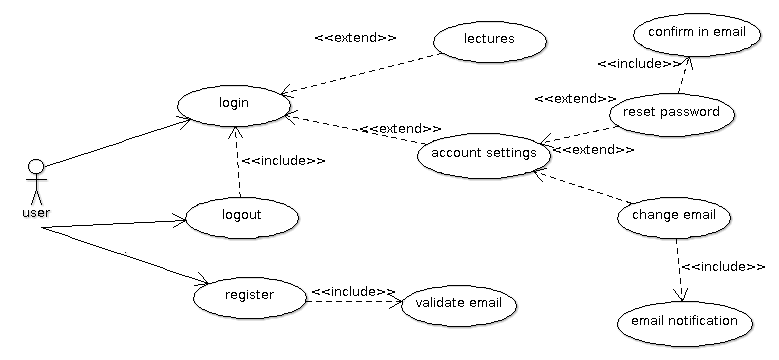
\includegraphics[width=0.8\textwidth, totalheight=6cm]{login_use_case}
	\caption{\textit{Prototype 1.0: Login Use Case}}
	\label{f3.5.1.1}
\end{figure}

%____________________________section____________________________
\section{Sequence Diagrams}\label{3.6}

\subsection{Prototype 1.0}\label{3.6.1}

\subsubsection{Register Sequence Diagram}\label{3.6.1.1}
\begin{figure}[!ht]
	\centering
		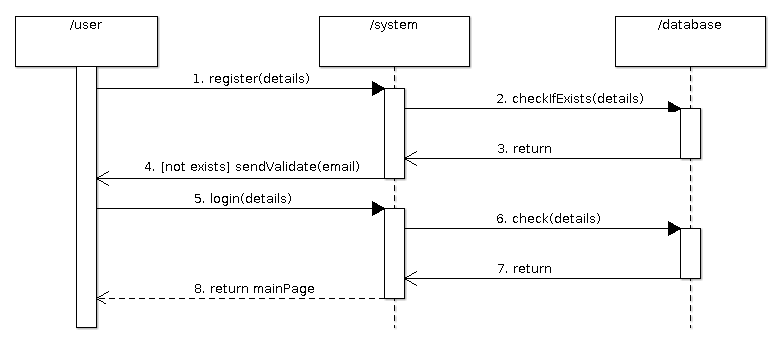
\includegraphics[width=0.8\textwidth, totalheight=5.5cm]{register_sequence_diagram}
	\caption{\textit{Prototype 1.0: Register Sequence Diagram}}
	\label{f3.6.1.1}
\end{figure}

\subsubsection{Account Settings Sequence Diagram}\label{3.6.1.2}
\begin{figure}[!ht]
	\centering
		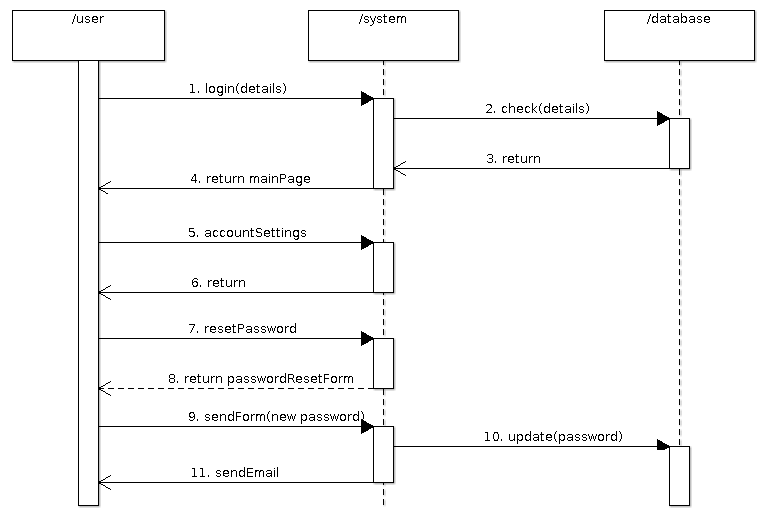
\includegraphics[width=0.8\textwidth, totalheight=6cm]{account_settings_sequence_diagram}
	\caption{\textit{Prototype 1.0: Account Settings Sequence Diagram}}
	\label{f3.6.1.2}
\end{figure}


%____________________________section____________________________
\section{User Interface Design}\label{3.7}

\subsection{Prototype 1.0}\label{3.7.1}

\subsubsection{Main Page Wireframe}\label{3.7.1.1}
\begin{figure}[!ht]
	\centering
		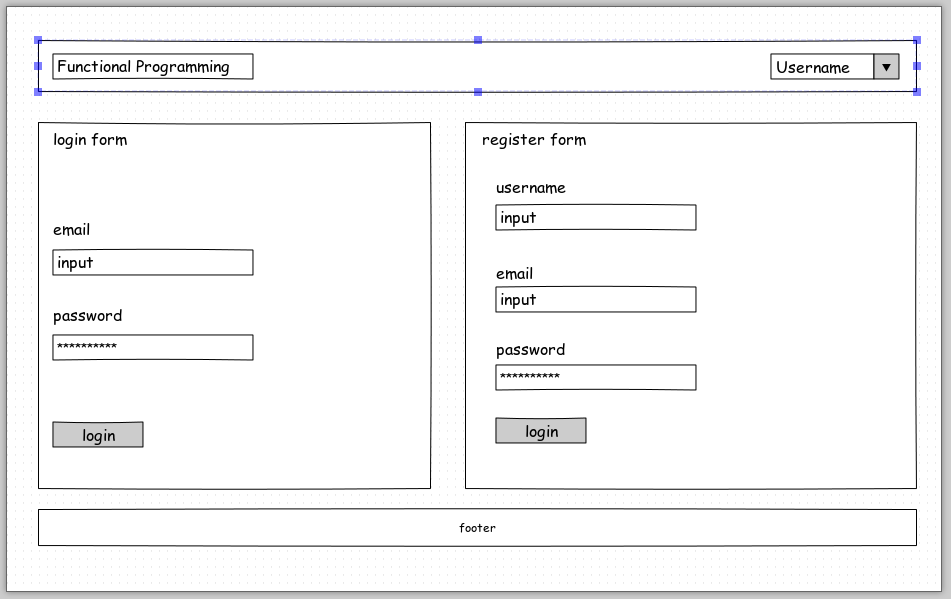
\includegraphics[width=0.8\textwidth, totalheight=7cm]
		{wireframe_main_page}
	\caption{\textit{Prototype 1.0: Main Page Wireframe}}
	\label{f3.7.1.1}
\end{figure}

On the main page, the user can log-in or register a new account. If the user attempts to log-in without the account, the attempt is rejected. The successful log-in will result in redirection to the dashboard page. Upon successful account registration, the user will receive the email with a confirmation link which he must click to validate the registration.

\textbf{Required Elements}
\begin{itemize}\itemsep1pt \parskip0pt \parsep0pt
\item header (label, hidden drop-down menu)
\item login form (labels, text input, password input, button)
\item register form (4 labels, text inputs, password input, button)
\item footer
\end{itemize}

\subsubsection{Dashboard Wireframe}\label{3.7.1.2}
\begin{figure}[!ht]
	\centering
		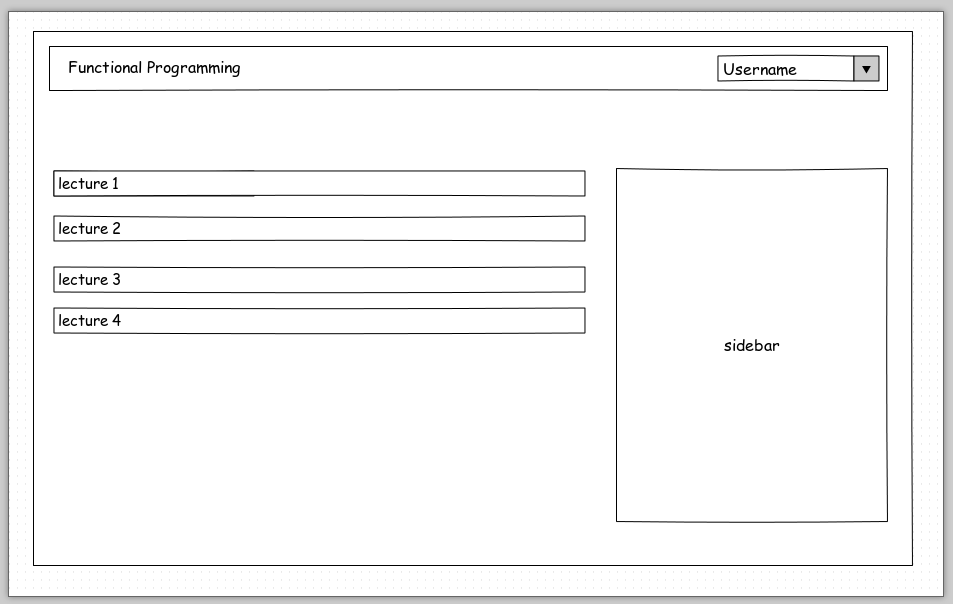
\includegraphics[width=0.8\textwidth, totalheight=7cm]
		{wireframe_dashboard}
	\caption{\textit{Prototype 1.0: Dashboard (lectures) Wireframe}}
	\label{f3.7.1.2}
\end{figure}

On the dashboard page user will have access to the lectures. Also, the drop-down menu in the header will be visible and will allow the user to request the account settings page or log-out. The account setting request will result in the account settings page redirection and the log-out request will result in the redirection to the main page.

\textbf{Required Elements}
\begin{itemize}\itemsep1pt \parskip0pt \parsep0pt
\item header (label, visible drop-down menu)
\item main area (links to the lectures)
\item side area (for future functionality)
\item footer
\end{itemize}

\subsubsection{Account Settings Wireframe}\label{3.7.1.3}
\begin{figure}[!ht]
	\centering
		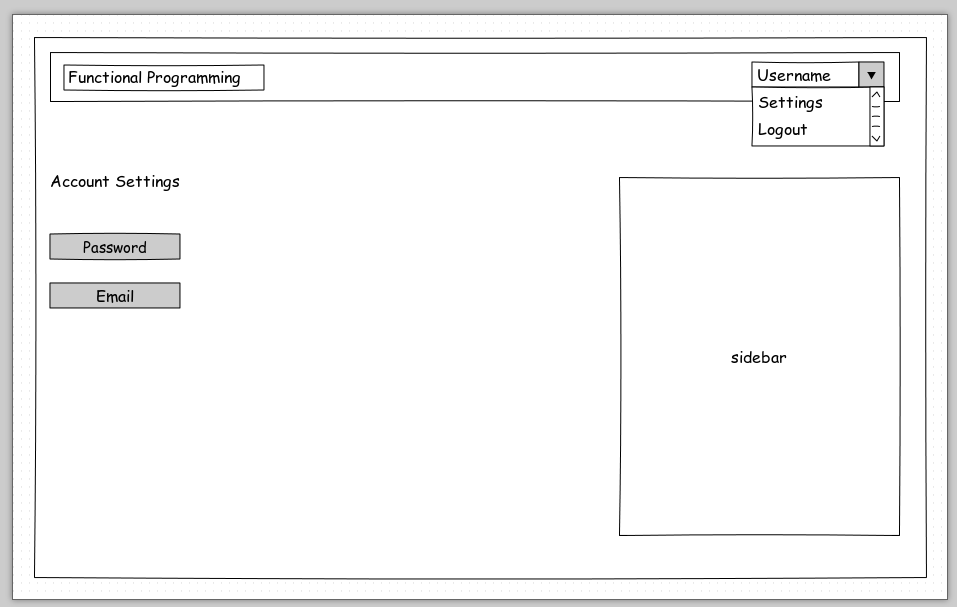
\includegraphics[width=0.8\textwidth, totalheight=7cm]
		{wireframe_account_settings}
	\caption{\textit{Prototype 1.0: Account Settings Wireframe}}
	\label{f3.7.1.3}
\end{figure}

On the account setting page, the user can change the password or the email address. Upon the password change request, the email will be sent to the user with the confirmation link. Upon the successful email change, the user will receive the notification email.

\textbf{Required Elements}
\begin{itemize}\itemsep1pt \parskip0pt \parsep0pt
\item header (label, visible drop-down menu)
\item main area (2 buttons)
\item side area (for future functionality)
\item footer
\end{itemize}

%____________________________section____________________________
\section{Database Schema Design}\label{3.8}

\subsection{Prototype 1.0}\label{3.8.1}
For the prototype 1.0 functionality, I will need the entity which will represent the user and the entity which will represent a random token. I will generate a token and associate it with the user every time a user requests registration, password change or email change. These tokens will then be embedded into an URL which will be sent to user's email. It's basically a way of identifying the user actions. The user then must click the URL to validate (confirm) the action. There should be a general expiration period associated with each token. Let's say one day. If the user doesn't confirm the requested action the action will be cancelled. For this functionality, I will need to save the token creation time-stamp as well.

\begin{figure}[!ht]
	\centering
		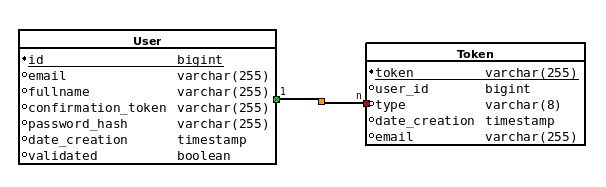
\includegraphics[width=0.7\textwidth, totalheight=6cm]
		{entity_relations_diagram1}
	\caption{\textit{Prototype 1.0: Entity Relations Diagram}}
	\label{f3.8.1}
\end{figure}

%____________________________section____________________________
\section{Back End Design}\label{3.9}

\subsection{Prototype 1.0}\label{3.9.1}
In Play! Framework the user interfaces are represented by views. The view consists of HTML, Javascript and embedded Scala\cite{30} code. The views are compiled to Scala classes and stored in /views folder. The views are rendered on demand by the server.

The user interacting with the views creates the requests to the resources. The incoming requests are handled by controllers. Each request is routed to the one controller method. Controller methods are processing the request and returning responses which in turn render the views. Controllers are stored in /controllers folder.

The requests are routed to the controllers by rules stored in /conf/routes file. In this file, the mappings form URIs to controller methods are defined. Play Framework uses REST like approach to routing. The /conf directory serves as a storage for all configuration files.

\begin{figure}[!ht]
	\centering
		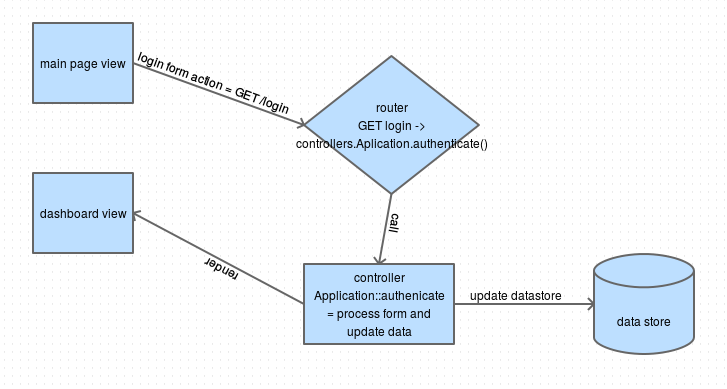
\includegraphics[width=0.8\textwidth, totalheight=7cm]
		{play_flowchart}
	\caption{\textit{View -> Request -> Controller -> Response -> View Diagram}}
	\label{f3.9.2}
\end{figure}

Play Framework is persistence agnostic, but it provides Java Ebeans ER mapper and H2 in memory database by default. H2 can be changed for other database implementation for the production mode and any other ER mapping framework can used instead of Ebeans. In Ebeans, the each entity is represented by a POJO annotated class called model. Models are stored in /models directory.

The layout of a Play application is standardized to keep things as simple as possible. After a first successful compile, a Play application looks like this:

\begin{figure}[!ht]
	\centering
		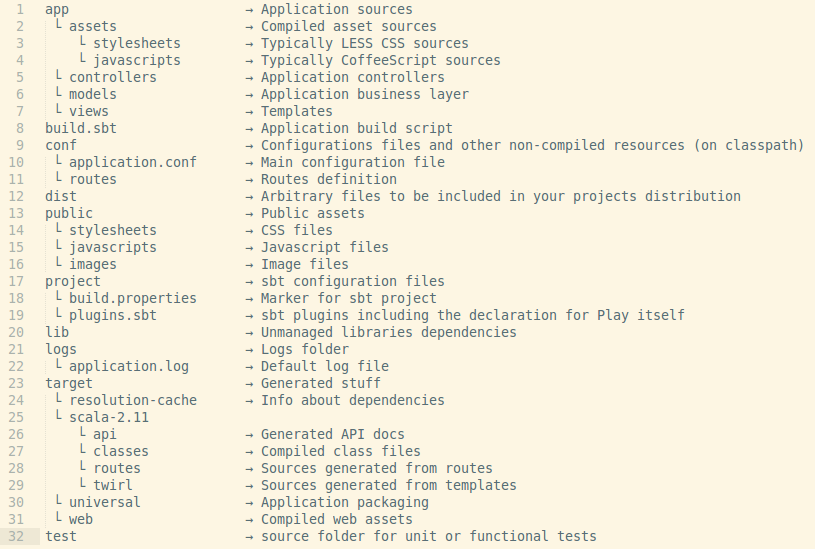
\includegraphics[width=1\textwidth, totalheight=10cm]
		{play_framework_project_anatomy}
	\caption{\textit{Play Framework Project Anatomy}}
	\label{f3.9.1}
\end{figure}

%____________________________section____________________________
\section{Project Repository Design}\label{3.10}
Project repository will be hosted on GitHub page: \url{https://github.com/zubidlo/itb_honours_project}.
I propose following directory structure:

\begin{figure}[!ht]
	\centering
		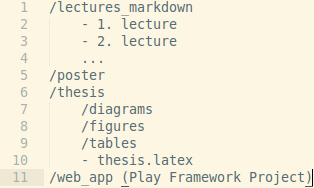
\includegraphics[width=0.4\textwidth, totalheight=4cm]
		{github_repo_anatomy}
	\caption{\textit{GitHub Repository Anatomy}}
	\label{f3.10}
\end{figure}


%____________________________section____________________________
\section{Conclusion}\label{3.11}
It this section I discussed the preliminary design of the project. I argued that the prototyping software development methodology would the appropriate approach in the development of this project. I outlined the form the learning material should take and I decided to use Scala programming language to communicate functional programming ideas in code.

The web application publishing the learning material for students will be developed using Play! Framework. The application design will follow the standardized anatomy of a Play application and I will use Git as versioning system and GitHub repository to store the project. Play supports both Java and Scala programming languages and I have not yet decided what programming language I will use to develop the application. Also, I listed all the tools I will use in the project implementation.

With the help of UML, I outlined proposed design for web application prototype version 1.0. In this prototype iteration, the application will support user log-in and registration, account settings and log-out. The application will require email validation with expiration date and password should be stored as encrypted hashes. The application will also list all the learning material and reserve a space for an additional functionality.










%_______________________________chapter_______________________________________
\chapter{Implementation}\label{4}

%____________________________section____________________________
\section{Introduction}\label{4.1}
In this section, I will discuss some of the web application implementation details. As outlined in chapter \ref{3.9.1} the application will be rendered on the server side and will consist of views, routes, controllers, and models. The views are basically HTML pages returned by the server on user requests. They are all the user is seeing and interacting with.

\begin{figure}[!ht]
	\centering
		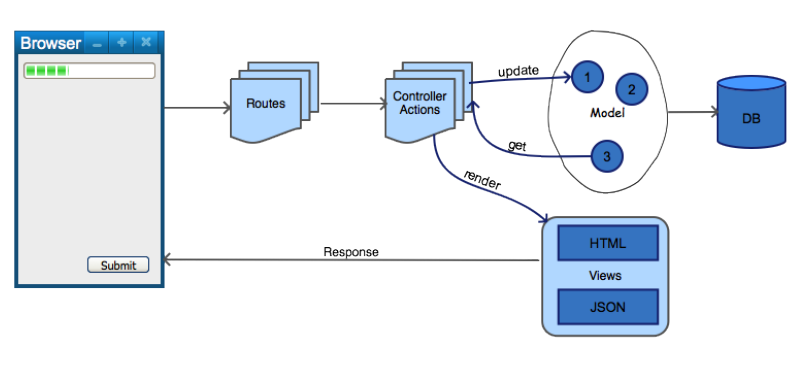
\includegraphics[width=0.7\textwidth, totalheight=5.8cm]
		{play_workflow_diagram}
	\caption{\textit{Play WorkFlow Diagram}}
	\label{f4.1}
\end{figure}

The rest of the Play infrastructure is working in "the background" to make sure that views are returned to user filled with appropriate data. The router routes the requests such as an HTML form POST action to a controller method which will process the form. For example, log-in form POST request will be routed to the appropriate controller method, which will first validate the form. Next, the user data will be fetched from the model and compare to the data in the form. If there is a match, the controller method will render the dashboard view and send it back to the user. Also, the server will maintain the session during the user interaction with the views as long as the user is logged-in.

The application will be developed locally on a laptop and deployed on a live internet server. I chose Microsoft Azure Cloud for the deployment.  The reason is that I already have the access to the Azure and I'm familiar with the service management console.

%____________________________section____________________________
\section{Development Set-Up}\label{4.2}
The Play Framework is the part of Lightbend Reactive Platform\cite{32}. The platform uses Lightbend Activator User Interface for the development. The user installs the activator locally and starts the service. The user interface is spawned in the browser (figure \ref{f4.2}) in which user can create new web application or develop, build, run and test existing web application. I used activator and eclipse for the application development.

The new application development doesn't start from scratch, but user rather creates a new application by choosing one of 400 templates. These templates are scaffolds consisting of standardized Play project directory structure and already imported libraries required for chosen type of the web application. Also, the templates serve the role of tutorials for the beginners. I created the new Play Java application from a template tutorial showcasing the user log-in and I imported additional Javascript libraries for user interface enhancement such as Scala code highlighting.

\begin{figure}[!ht]
	\centering
		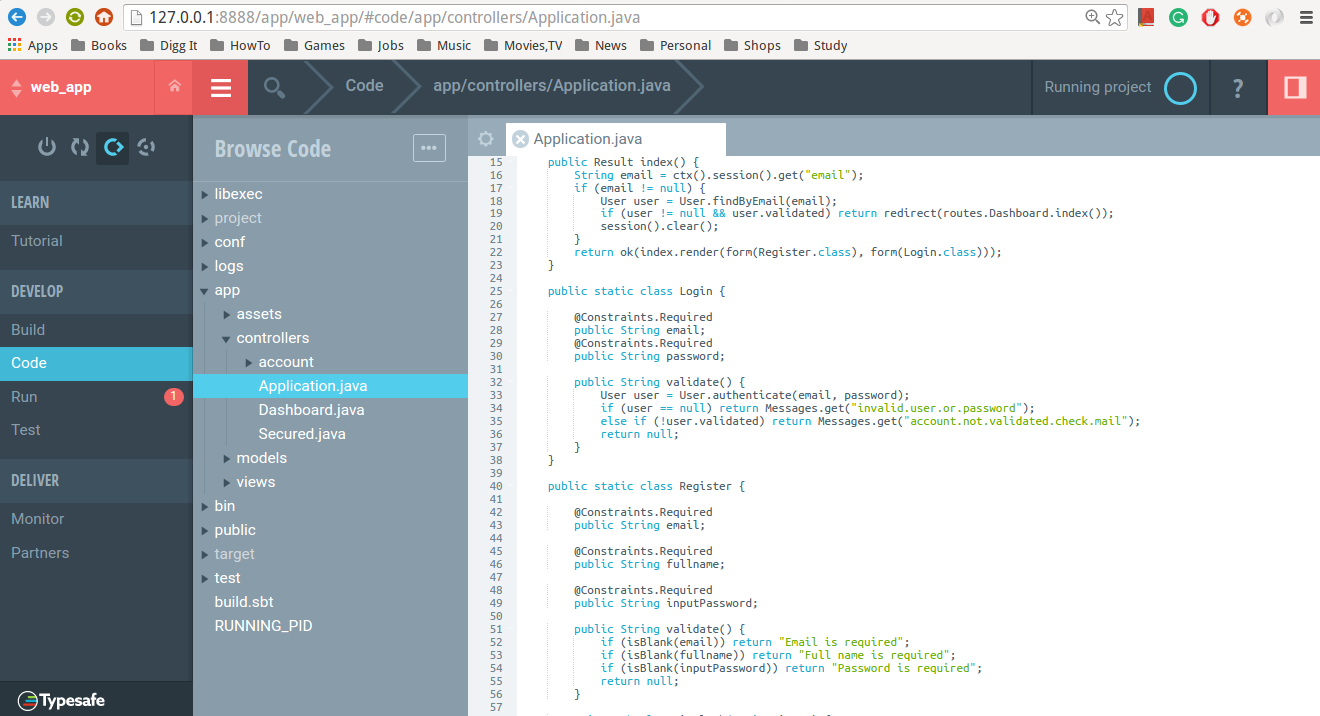
\includegraphics[width=0.9\textwidth, totalheight=8cm]
		{activator}
	\caption{\textit{Lightbend Activator}}
	\label{f4.2}
\end{figure}

To start an application development from a template is not specific just to Play Framework, but it is a common practice in most of the web application development platforms. Java EE and .NET offer the same functionality. Because I'm an absolute beginner in Play web application development I found this approach very useful. I choose the template which is in turn extension of \url{https://www.playframework.com/documentation/2.2.x/JavaGuide1} tutorial.

There is a slight issue with Play approach to backward compatibility. The current Play version I installed is 2.5 and the template and tutorial I followed are working with the version 2.2. Play Framework evolved quite a bit between the versions and there are migration steps need to take place to ensure the application is working. Play documentation includes migration guides, but it is mandatory to follow migration guide from version 2.2 to version 2.3, then from 2.3 to 2.4 and finally from 2.4 to 2.5, which effectively requires a study of Play Framework evolution. 

%____________________________section____________________________
\section{User Interfaces (Views)}\label{4.3}

The user interface is contained in package "views". The views are developed with usage of Scala templates. Each view is compiled to the Scala object and the HTML can be then rendered by calling the render() method on the given view object. This action is usually done in a controller method as the last step before the rendered HTML is inserted in the response. The view can be arbitrary nested, allowing for creating common layouts (header, footer) just once. The views can carry state-full information as well, such as references to some useful values existing outside the views. This can be used to maintain the session state for example. Every view must have a reference to a user object, which gets created when a user successfully logs in. In the case the user object is not available, a view will redirect to the index page. This way only the logged-in user would get an access to certain views.

\subsection{Prototype 1.0}\label{4.3.1}

\subsubsection{Main Layout View}\label{4.3.1.1}
The main layout view consists of a header (navigation bar) and footer. References to the User and additional HTML @content are imported at the top of the view. Every additional view is then inserted on @content placeholder. Also, scripts and CSS are imported in this view.

\begin{figure}[!ht]
	\centering
		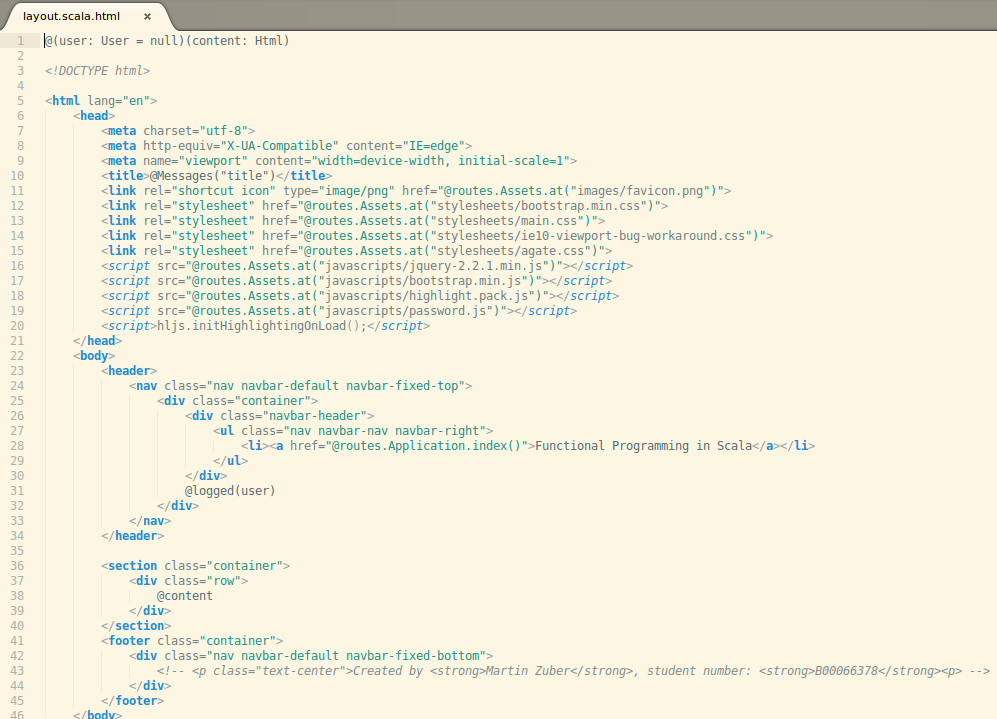
\includegraphics[width=0.9\textwidth, totalheight=8cm]
		{main_layout_view}
	\caption{\textit{Main Layout View}}
	\label{f4.3.1.1}
\end{figure}

\subsubsection{Index View}\label{4.3.1.2}
The index view consists of 2 forms, the login and register form. The view is inserted into main layout view and rendered by the server as the main page of the web application.

\begin{figure}[!ht]
	\centering
		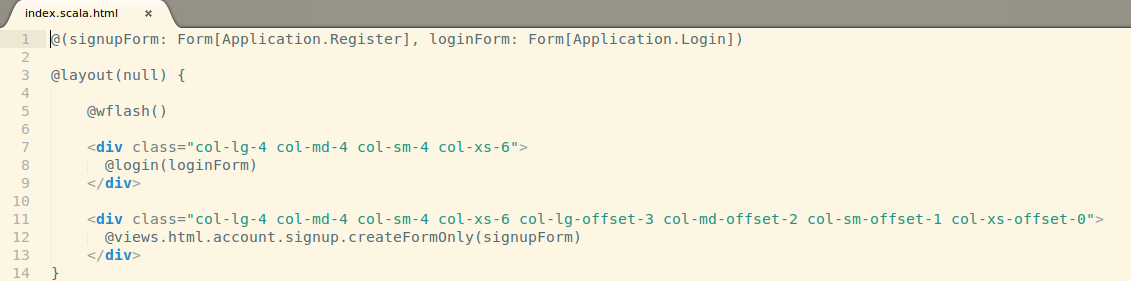
\includegraphics[width=0.9\textwidth, totalheight=4cm]
		{index_view}
	\caption{\textit{Index View}}
	\label{f4.3.1.2}
\end{figure}

The figure \ref{f4.3.1.3} is a snapshot of the rendered main page.

\begin{figure}[!ht]
	\centering
		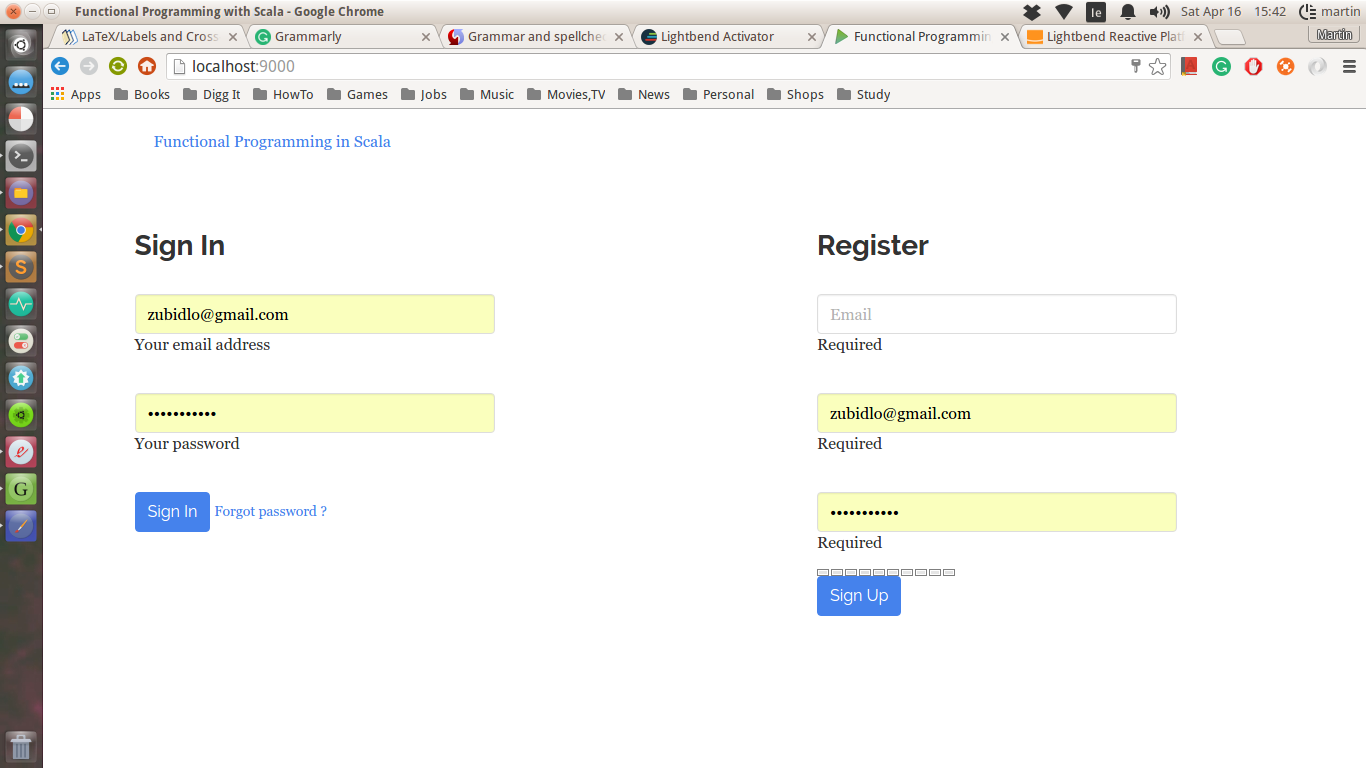
\includegraphics[width=0.9\textwidth, totalheight=8cm]
		{main_page_view}
	\caption{\textit{Main Page}}
	\label{f4.3.1.3}
\end{figure}

All the user interface implementations in Prototype 1.0 are following this pattern. The layout view is a container in which appropriate views are inserted in. This nested view is then rendered into HTML.

\subsubsection{Password Strength}\label{4.3.1.3}
Each form which contains the password input field is enhanced with animated success bar like control under the field. The bar is mimicking the password strength as the user writing the password in the field. This functionality was taken from \url{http://benjaminsterling.com/wp-content/files/passwordstrength.htm} and consists of \emph{assets/javascript/password.coffee} and \emph{assets/styles/main.less} files. The important fact is that Play Framework compiles \emph{coffee scripts} into \emph{javascript} and \emph{less} into css sheets during the compilation.

\subsubsection{Internationalization}\label{4.3.1.4}

Play follows the common I18N scheme to address the internationalization. The developer specifies the languages using language tags, such as "en" for English. These are defined in \emph{conf/application.conf} file by:
\begin{lstlisting}[language=java]
	play.i18n.langs = [ "en", "en-US", "fr" ]
\end{lstlisting}

The text is externalized to text files \emph{conf/messages.en}, \emph{conf/messages.fr} and so on. The message text file consists of simple mappings:
\begin{lstlisting}[language=java]
	title=Functional Programming with Scala
	files.summary=The disk {1} contains {0} file(s).
\end{lstlisting}
which are referenced from Java by:
\begin{lstlisting}[language=java]
	Messages.get("title")
	Messages.get("files.summary", d.files.length, d.name)
\end{lstlisting}

The current language is found by looking at the \emph{lang} field in the current Context and can be changed at any time. The Context’s \emph{lang} value can be determined by other means:
\begin{enumerate}\itemsep1pt \parskip0pt \parsep0pt
\item Context’s lang field explicitly
\item \emph{PLAY\_LANG} cookie in the request header
\item the \emph{Accept-Language} headers of the request
\item the application’s default language
\end{enumerate}

%____________________________section____________________________
\section{Data And Helper Classes (Models)}\label{4.4}
The model package consist of Ebean entities and some useful utility helper classes. Ebean framework supports common JPA annotations for entities and simple fluent API for handling database updates.

\begin{lstlisting}[language=java]
	FIND.where()
		.eq("email", email)
		.findUnique();
\end{lstlisting}

In this example the chained call will return the user with given address or null. FIND is a reference to model.Finder class which handles User entity.

\subsection{Prototype 1.0}\label{4.4.1}
The model package in this prototype iteration consist of following classes:
\begin{itemize}\itemsep1pt \parskip0pt \parsep0pt
	\item User
	\item Token
	\item package utils
	\begin{enumerate}\itemsep1pt \parskip0pt \parsep0pt
	\item AppException
	\item Hash
	\item Mail
	\end{enumerate}
\end{itemize}

\subsubsection{User}
The User class is annotated JPA Entity which directly maps to User database table. The class has a set of static methods which allow to find a user by email or by the confirmation token, authenticate the user, change user password and confirm the user.

\subsubsection{Token}
The Token is annotated JPA Entity which directly maps to the Token database table. Token functionality allows to create a new token and to find already existing token. The token purpose is to enable email confirmation functionality for registering the new account, resetting the password or changing email of an existing account.

\textbf{Token usage in password reset workflow:}

\begin{enumerate}\itemsep1pt \parskip0pt \parsep0pt

\item User clicks on "Reset" button beside "Password" label in the account settings view. This button is "submitting" empty form with POST action which matches \emph{runPassword() of Password} controller method.
	\begin{lstlisting}[language=java]
	POST    /settings/password   controllers.account.settings.Password.runPassword()
	\end{lstlisting}
	
	\item Method runPassword () will check if there is \emph{email} stored in the current session and if so the user with this email address will be fetched from the database, the new genuine token will be created and associated with the user and email with the confirmation link will be sent to the email address.
\begin{lstlisting}[language=java]
	@Security.Authenticated(Secured.class)
    public Result runPassword() {
        User user = User.findByEmail(request().username());
        try {
            Token t = new Token();
            t.sendMailResetPassword(user, mailerClient);
            flash("success", Messages.get("resetpassword.mailsent"));
            return ok(password.render(user));
        } catch (MalformedURLException e) {
            flash("error", Messages.get("error.technical"));
        }
        return badRequest(password.render(user));
    }
\end{lstlisting}
\textbf{Notice:} Play Framework is binding every request to the Request object. The request object can be retrieved by calling Controller:: request () method. The Request object represents an HTTP request with header and body, but it has an additional \emph{username} field, which can be set at any time. This field serves as an authentication mechanism. In this application design the \emph{@Security.Authenticator} controller injects the \emph{email} address from the current session into the request.username field assuming that during an user log-in his email address was stored in the session. This way Play allows me to identify each request with a logged-in user.

\item The user receives the email asking him to click on \url{ http://localhost:9000/reset/61ec0e88-9db6-4103-bf9d-d299ba03f9f8} to reset the password. This link includes the immutable universally unique identifier (UUID) of the created token and matches following route:
\begin{lstlisting}[language=java]
 GET   /reset/:token   controllers.account.Reset.reset(token: String)
\end{lstlisting}
When user clicks on the link the Reset::reset(String token) controller method will be invoked.

\item The reset() method will check if given token exists, if it is of token type used for resetting passwords and if the token is not expired. The tokens expire in one day. If everything is right, the password reset view is rendered and reset form and the token is passed to it.

\item In the reset view the user input his new password in the form and on the form submission the form post matches:
\begin{lstlisting}[language=java]
 POST   /reset/:token   controllers.account.Reset.runReset(token: String)
\end{lstlisting}
and Reset::runReset(String token) controller method is invoked with token as the argument.

\item The runReset () method will again validate the token as before in reset() method and if that is successful the user will be fetched from the database based on the token userId field and his password will be updated. The confirmation email will be then sent to user email account and the control will be redirected to dashboard view.
\end{enumerate}

\subsubsection{AppException}
The AppException is just a simple exception class, which allows me to create custom exceptions.

\subsubsection{Hash}
The Hash is a collection of two static methods which uses org.mindrot.jbcrypt\cite{35} library to encrypt and decrypt the passwords.

\begin{lstlisting}[language=java]
 package models.utils;

import org.mindrot.jbcrypt.BCrypt;

public final class Hash {

    public static String createPassword(String clearString) throws AppException {
        if (clearString == null) throw new AppException("No password defined!");
        return BCrypt.hashpw(clearString, BCrypt.gensalt());
    }

    public static boolean checkPassword(String candidate, String encryptedPassword) {
        if (candidate == null) return false;
        if (encryptedPassword == null) return false;
        return BCrypt.checkpw(candidate, encryptedPassword);
    }
}
\end{lstlisting}


\subsubsection{Mail}
The Mail class is the implementation of email client using Play built-in email support library. The emails are build and send from a separate thread one second after the thread is started. Play includes very powerful support for concurrency in the form of Akka toolkit.\cite{33} Akka is an award winning open source project for building highly concurrent,
distributed, and resilient message-driven applications on the JVM based on Scala Actors threading model. Akka is capable of handling 50 million msg/sec on a single machine with a small memory footprint with ~2.5 million actors per GB of the heap.

The Mail client uses dedicated email account at \url{functional.scala@gmail.com} to send emails to users. The connection is done through SMTP protocol over SSL with and port number 456.

In the case of a user registration processing the Signup:: sendMailAskForConfirmation controller method creates a new random token and assigns it to the new user. The email message is then constructed which includes a link such as \url{ HTTP://localhost:9000/confirm/5ef75942-86ba-4841-a413-70126f9d8e65}. Clicking on this link will resolve in route to the \emph{controllers.account.Signup.confirm(confirmToken: String)} controller method which will validate the new user account and send the confirmation email.

\begin{figure}[!ht]
	\centering
		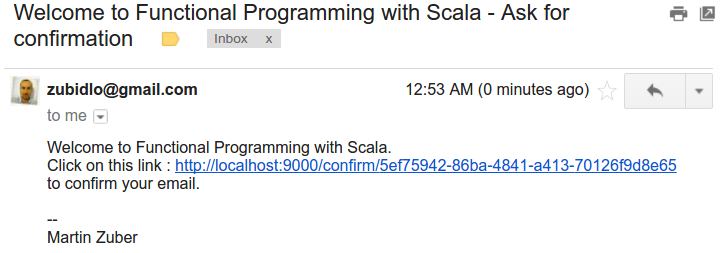
\includegraphics[width=0.9\textwidth, totalheight=4cm]
		{register_confirmation_email}
	\caption{\textit{Validate New Account E-mail}}
	\label{f4.4.1.1}
\end{figure}

\begin{figure}[!ht]
	\centering
		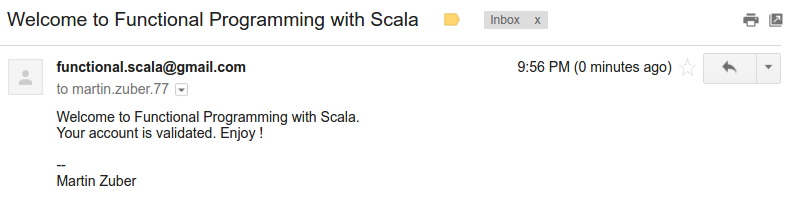
\includegraphics[width=0.9\textwidth, totalheight=4cm]
		{register_notification_email}
	\caption{\textit{Validate New Account E-mail}}
	\label{f4.4.1.2}
\end{figure}


%____________________________section____________________________
\section{Business Logic (Controllers)}\label{4.5}
As outlined in section \ref{4.1} the user requests are routed to the controller methods. These methods consist all the business logic of the application. Each method is processing the request and creating the response which usually contains a new HTML page rendered from a view. The mappings from HTTP requests to the controller methods are stored in routes file.

\begin{lstlisting}[language=java]
	POST    /login     		controllers.Application.authenticate()
\end{lstlisting}

In the example above is the route from log-in form action to the corresponding controller method. When user triggers the log-in form action (POST) by clicking on Login button, the Application::authenticate method is invoked.

\begin{lstlisting}[language=java]
	public Result authenticate() {
        Form<Login> loginForm = form(Login.class).bindFromRequest();
        Form<Register> registerForm = form(Register.class);
        if (loginForm.hasErrors()) return badRequest(index.render(registerForm, loginForm));
        else {
            session("email", loginForm.get().email);
            return redirect(routes.Dashboard.index());
        }
    }
\end{lstlisting}

The authenticate method fetches data from the POST request body and bind them to the POJO class representing the form data (email, password). Because the index page has both forms, also an empty registration form is bound to it's POJO representation. The log-in form is then validated against the User model and if it contains errors the index page is rendered and send back to browser inside the badRequest response (code 400). From the user point of view, the index page is reloaded with error message included.

\begin{figure}[!ht]
	\centering
		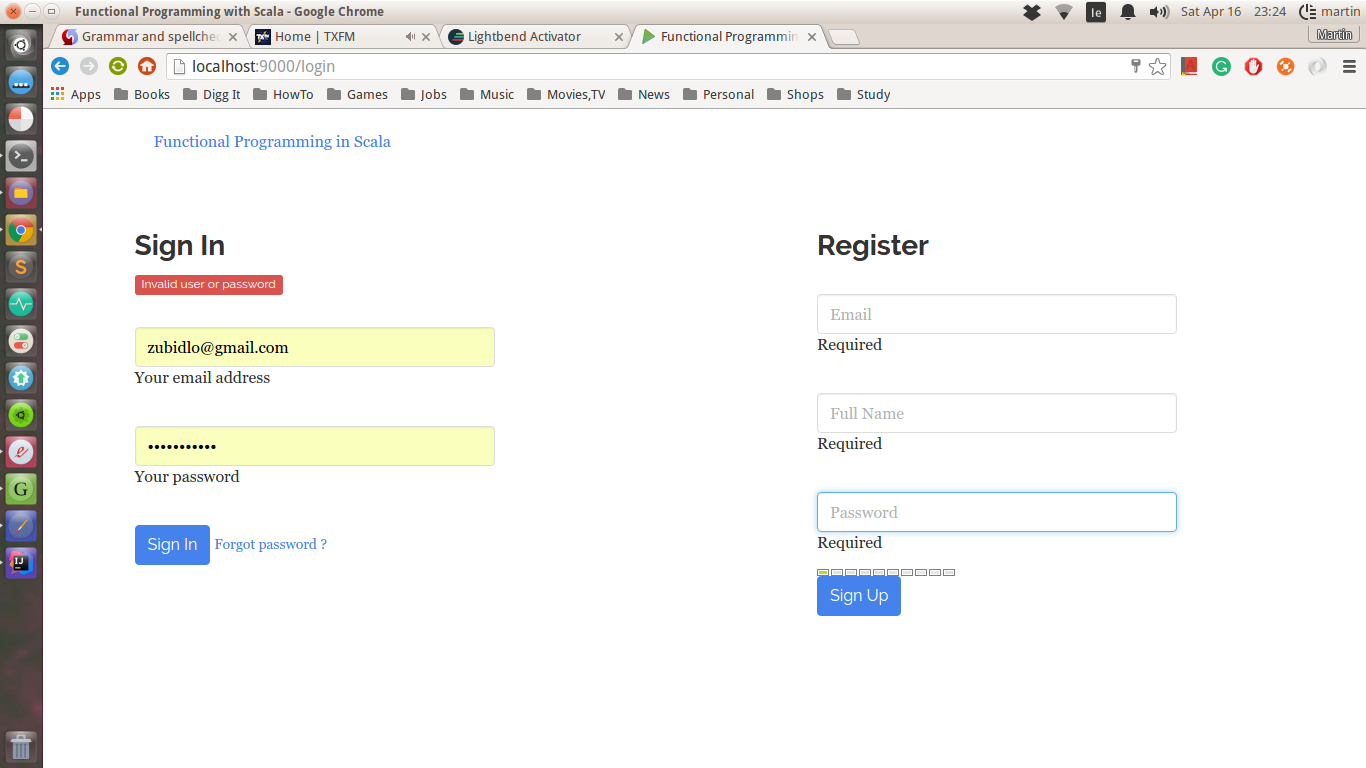
\includegraphics[width=1\textwidth, totalheight=8cm]
		{invalid_user_or_password_view}
	\caption{\textit{Unsuccessful Log-in Response}}
	\label{f4.5.1}
\end{figure}

In the case, the user log-in form contained valid email and password, the user's email is saved in the session storage and the user interface is redirected to dashboard view. The dashboard view can be only accessed as long as the session storage contains an email of a registered user or the session is not expired. Actually, every view which requires logged user is checking the session storage for valid email matching the existing user row in the database. In the case the session is empty the views redirect back to index page.

\subsection{Prototype 1.0}\label{4.5.1}

Figure \ref{f4.5.1.1} is a screenshot of all the routes in prototype 1.0 implementation. Special case is the last line:
\begin{lstlisting} [language=java]
	GET /assets/*file controllers. Assets. at (path="/public", file)
\end{lstlisting} 
which handles location of static assets such as CSS styles and script files stored in /public directory of the applications. These files must be handled as Java resources because in a production environment the application will be deployed as \textbf{.jar} archive.

\begin{figure}[!ht]
	\centering
		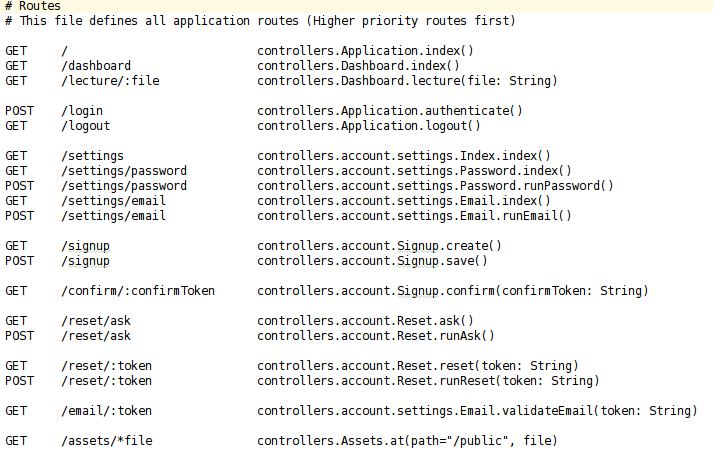
\includegraphics[width=1\textwidth, totalheight=9cm]
		{routes}
	\caption{\textit{Routes}}
	\label{f4.5.1.1}
\end{figure}

Controller classes are implemented in the Java programming language in this prototype iteration. The reason for this decision was purely pragmatic. Being Scala and Play beginner, I planned to learn the Play Framework in the first prototype implementation. In later iterations, I have planned to refactor all the Java code to Scala as soon as I would become comfortable enough with the new language. Scala is often referred to as the most evolved programming language on the planet and I soon found out that Play uses advanced Scala features such as \emph{imlicits}.

There has been enough complexity involved just with a study of Play Framework alone. After all, the main point of prototyping approach to a software development is to be able to have a working prototype as soon as possible.

%____________________________section____________________________
\section{Deployment}\label{4.6}
The application is deployed on Azure Cloud Virtual Machine \url{http://martinzuber.cloudapp.net/}. Play Framework doesn't require an application server for deployment. Play includes its own HTTP server and is deployed as the standalone application. Activator creates distribution version.zip archive which contains the startup script. This archive can be then copied to live server, unpacked and run.

\subsection{Required Steps for Deployment Set-Up}\label{4.6.1}

\subsubsection{1. Create a virtual machine.}
Azure cloud offers classic virtual machines. The user chooses data centre location, a number of processor cores, memory size, disk size, and bandwidth. The selection will dictate the price per month. Virtual machine specifications can be adjusted dynamically later if the requirements change. For example, the machine can be migrated to a different geographical location, cores, memory can be added and so on. Microsoft offers a wide range of pre-configured operating system images to be installed automatically during the machine creation. The user can choose from quite a rich selection of Linux distribution images and specialized appliances are available as well. All images come with configured SSH server.

Deployment Virtual Machine Specifications:
\begin{itemize}\itemsep1pt \parskip0pt \parsep0pt
\item Type: Basic A1 (1 Core, 1.75 GB memory)
\item OS: Ubuntu Server 14.04 LTS
\item Location: Europe North (Dublin West Data Centre)
\item DNS name: martinzuber.cloudapp.net
\item Public Virtual IP: 40.85.129.158
\end{itemize}

\subsubsection{2. Install and configure all required software}
To be able to deploy Play web application I need to install following software:
\begin{itemize}\itemsep1pt \parskip0pt \parsep0pt
\item Java SE Platform
\item MySQL database
All the Play distribution build needs is installed Java SE Platform. Netty server and all the dependencies are included in the build. The H2 in-memory database will be replaced by MySQL in production when the application is fully developed.
\end{itemize}

\subsubsection{3. Configure Endpoints.}
Endpoints are mappings from Azure internet facing ports to internal ports on the virtual machine. For example, to be able to connect to the machine with SSH protocol, the following endpoint must be created:
\begin{lstlisting} [language=bash]
	name: SSH, protocol: TCP, public port: 22, private port: 22
\end{lstlisting}
This endpoint would make virtual machine port 22 available from the outside the cloud. I configured the following endpoints:

\begin{figure}[!ht]
	\centering
		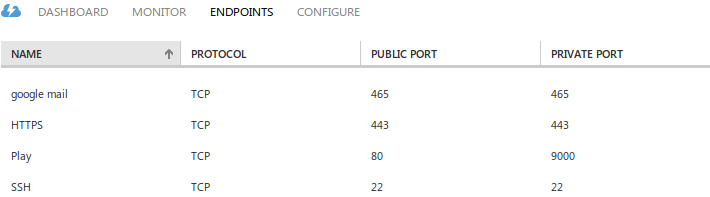
\includegraphics[width=1\textwidth, totalheight=4cm]
		{endpoints}
	\caption{\textit{Virtual Machine Endpoints}}
	\label{f4.5.1}
\end{figure}

\subsubsection{4. Create and configure web app distribution build.}
Even though to create the production build in Play is a question of one activator command, the necessary changes have to be made in the production build configuration:
\begin{enumerate}\itemsep1pt \parskip0pt \parsep0pt
\item The web application is sending emails consisting of a URL to validate user actions such as account registration as I discussed in the section \ref{4.4.1}. When the application is deployed its domain name changes and so must the URL in those emails. The domain name is therefore not hard-coded, but rather stored in the \emph{conf/application.conf} file and referenced from the code by name.
\begin{lstlisting} [language=java]
	server.hostname="martinzuber.cloudapp.net"
\end{lstlisting} 
\item Java Ebean ORM supports the database evolutions. This functionality allows having different database schema for each prototype or build. The schemas are stored in \emph{conf/evolutions/} directory and with each restart of the application, the developer is asked to choose an appropriate schema. This functionality is not allowed in the production mode and the database must be configured with the default schema at application start-up:
\begin{lstlisting} [language=bash]
	/path/to/web_app/app -Dplay.evolutions.db.default.autoApply=true
\end{lstlisting} 
or turned off in \emph{conf/application.conf} file:
\begin{lstlisting} [language=java]
	evolutions=disabled
\end{lstlisting} 
\item Application in production mode requires a private secret key. The key is used for signing session cookies, CSRF tokens and in built-in encryption utilities. Anyone with the access to the secret key can generate any session they please, effectively allowing them to log into the app. Therefore is highly recommended to store the key only on the production server and not to check the secret to source control. Also, if there are more instances of the application deployed the secret key must be the same for each instance. The secret key can be created in activator console with:
\begin{lstlisting} [language=bash]
	playGenerateSecret
\end{lstlisting}
and stored in \emph{conf/application.conf} by:
\begin{lstlisting} [language=java]
	play.crypto.secret="</N_v`W4xv8GY^c7e=UCDYF]vXSguUvABIHoi[JNm1j@lf2C6S9TL[?FNM?ImDd;"
\end{lstlisting}
\item In the development mode, the Play application uses H2 in-memory database, which only store data for the application runtime and schemes are deleted with each restart. The H2 driver configured in \emph{conf/application.conf} by:
\begin{lstlisting} [language=java]
	db.default.driver=org.h2.Driver
	db.default.url="jdbc:h2:mem:play"
\end{lstlisting}
In the production mode, MySQL server could used instead so the data are truly persistent.
\begin{lstlisting}[language=java]
	db.default.driver=com.mysql.jdbc.Driver
	db.default.url="jdbc:mysql://localhost/playdb"
	db.default.username=playdbuser
	db.default.password="a strong password"
\end{lstlisting}
\item As seen in steps 1-4, the production build differs from development in configuration of multiple items. For these cases Play provides an option to specify different configuration file for the production environment in the form of a command line argument:
\begin{lstlisting} [language=bash]
	/path/to/web_app/app -Dconfig.file=/full/path/to/conf/application-prod.conf
\end{lstlisting}
\end{enumerate}

\subsubsection{5. Create Upstart service.}
In Ubuntu 14.04, Upstart is a replacement for traditional \emph{init daemon} and it is responsible for bringing the computer into a normal running state after the boot-up. Upstart handles the starting, stopping and monitoring processes while the operating system is running. For each process to be managed by the Upstart daemon the .conf script must be created and stored in \emph{/etc/init/} directory. Processes defined by these scripts are called services.

I wrote following Upstart script \emph{/etc/init/play.conf} which turned the web app into a service daemon. The service is  started automatically at server startup as soon as the file system and network interface are alive. Also, running Play application stores its process id (PID) in a file which has to be deleted before the application can be restarted.

\begin{lstlisting} [language=bash]
	description "My Play Application"

	env USER=martin
	env GROUP=martin
	env APP_HOME=/home/martin/web_app-1.0-SNAPSHOT
	env APP_NAME=web_app               
 
	env EXTRA=""
 
	start on (filesystem and net-device-up IFACE=eth0)
	stop on runlevel [!2345]
 
	respawn
	respawn limit 30 10
	umask 022
	expect daemon
 
	pre-start script
    	#If improper shutdown and the PID file is left on disk delete it so we can start again
    	if [ -f $APP_HOME/RUNNING_PID ] && ! ps -p `cat $APP_HOME/RUNNING_PID` > /dev/null ; then
        	rm $APP_HOME/RUNNING_PID ;
    	fi
	end script
 
	exec start-stop-daemon --pidfile ${APP_HOME}/RUNNING_PID --chdir ${APP_HOME} --chuid $USER:$GROUP --exec ${APP_HOME}/bin/$APP_NAME --background --start -- -Dplay.evolutions.db.default.autoApply=true $EXTRA
\end{lstlisting}
The Upstart script syntax validity can be checked with:
\begin{lstlisting} [language=bash]
$ init-checkconf /etc/init/play.conf
\end{lstlisting}
The Play web application can be managed from terminal with commands:
\begin{lstlisting} [language=bash]
$ service start | stop | restart | status
\end{lstlisting}


%____________________________section____________________________
\section{Conclusion}\label{4.7}
In implementation chapter, I started with the description of a general structure of every Play application and how the pipeline from user interface toward the persistence storage is designed in the framework. In the comparison with multi-layered Java EE platform, the Lightbend Reactive Platform feels lightweight but more powerful.

Scala Twirl templates are closer to .NET Razor templates then to Java Server Faces. The templates are compiled to Scala objects and therefore are type-safe with the support of all the language features. On the other hand, they should handle only simple tasks and all the business logic is placed in the controller actions.

The requests coming from views are routed to controller methods which return responses usually in a form of another view. Play follows Model-View-Controller architectural pattern, but with REST-like resource oriented design. This approach feels very natural and logical. The framework is persistence agnostic and comes with default EBeans ORM mapper and various database drivers.

With each change in the code, the web application is recompiled and if compilation or runtime errors are printed in the browser window in development settings. Everything in Play application is therefore statically typed code. Play supports coffee script and less compilation as well.

The last section of the implementation chapter was dedicated to the application deployment in a lot of detail. The reason for such a detailed description was to document the process for a future reference. Overall, I had a quite positive experience using Azure cloud services.









%_______________________________chapter_______________________________________
\chapter{Testing and Evaluation}\label{5}

%____________________________section____________________________
\section{Introduction}\label{5.1}
Testing is an imperative part of any software development project. Eradicating errors and bugs is vital to the user experience. The successful test on one which identifies the bug in the application. There are various testing strategies to be performed:
\begin{itemize}\itemsep1pt \parskip0pt \parsep0pt
\item Unit testing – testing of a single function, procedure. The test subject is treated as a "black box" meaning that we test the subject functionality not the underlying implementation.
Integration testing – checks that units tested in isolation work properly when put together.
\item System testing – the emphasis is to ensure that the whole system can cope with real data, monitor system performance, test the system’s error handling and recovery.
\item Regression Testing – checks that the system preserves its functionality after maintenance and/or evolution tasks.
\item Acceptance Testing – checks if the overall system is functioning as required. It is usually performed by the end user on working application prototype.
\end{itemize}

The Play Framework comes with automated testing capabilities powered by the sbt build tool. Test classes are to be located in \emph{/test} directory and every method annotated with @Test will be included in the test run. The test can be run with "\emph{\$ activator test}" command or performed in the activator user interface.

\begin{figure}[!ht]
	\centering
		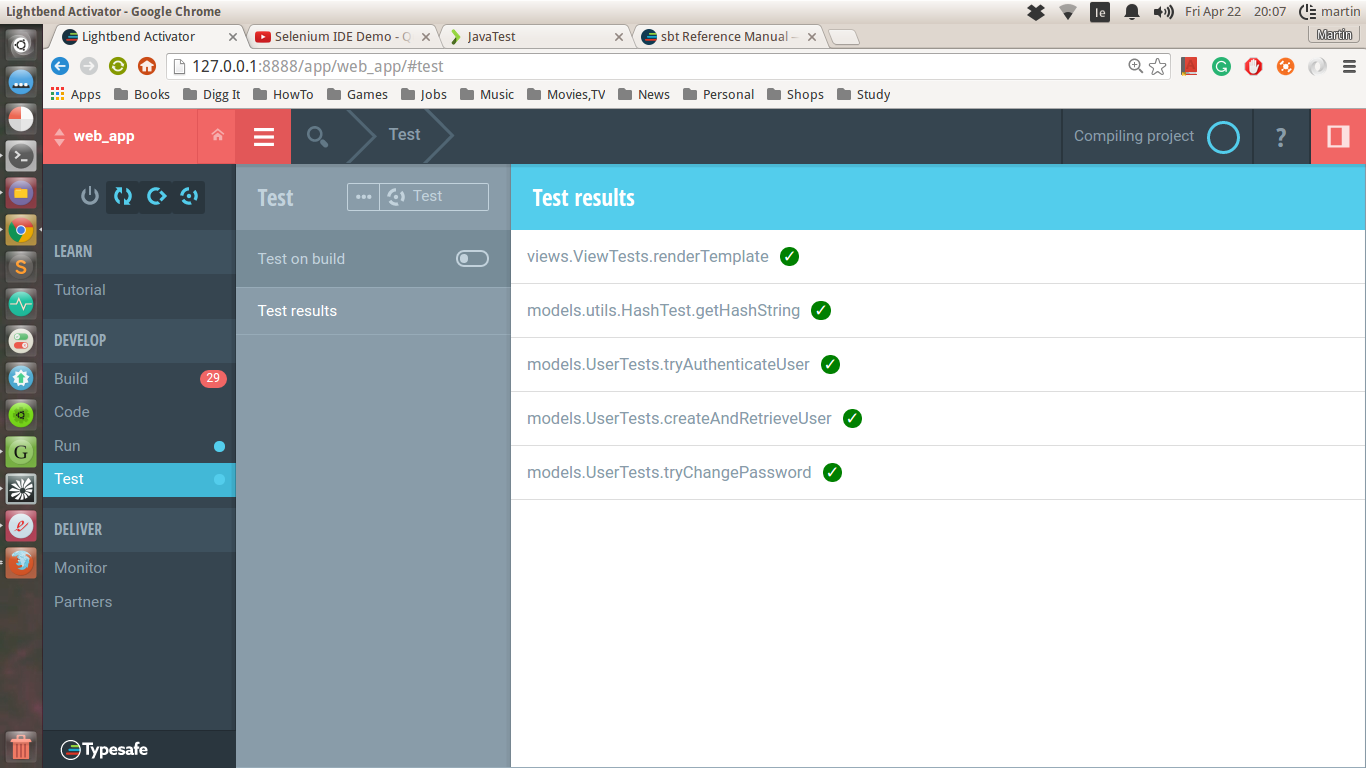
\includegraphics[width=1\textwidth, totalheight=9cm]
		{activator_test_run}
	\caption{\textit{Activator test run}}
	\label{f4.1.1}
\end{figure}

The Play Framework supports various test frameworks out of the box with the additional functionality of so called test helpers. Test helpers help to create mock instances of various Play components such as application, router or controller to make possible to test a component in isolation. Play comes with JUnit, WebDriver, ScalaTest support, but any testing framework can be used if needed.

In my test suite, I will concentrate to unit test the application models and utilities with JUnit test tool and test the user interface with Selenium IDE. In the following sections I will outline my approach to testing and discuss every found bug.

%____________________________section____________________________
\section{Unit Tests of Models and Utilities}\label{5.2}
Test are stored in \emph{/test/models} directory of the web application project. All test for an unit will be contained in one class.

\subsection{Prototype 1.0}\label{5.2.1}
\subsubsection{Hash}\label{5.2.1.1}
\begin{lstlisting}[language=java]
@Test
public void getHashString() throws AppException {
        
    String password = Hash.createPassword("hello world");
    Assert.assertNotNull(password);

    boolean matches = Hash.checkPassword("hello world", password);
    Assert.assertTrue(matches);

    boolean badPassword = Hash.checkPassword("some other password", password);
    Assert.assertFalse(badPassword);
}
\end{lstlisting}

\subsubsection{User}\label{5.2.1.2}

\begin{lstlisting}[language=java]
public class UserTests extends WithApplication {
	private String token;
	private User user;
    @Before
    public void setUp() throws AppException {
        start(fakeApplication(inMemoryDatabase()));
        String hash = Hash.createPassword("password1");
    	token = UUID.randomUUID().toString();
    	user = new User("martin@gmail.com", "Martin Zuber", hash, token);
    	user.save();
    }
    
    @Test
    public void createAndRetrieveUser() {
    	User martin = User.findByEmail("martin@gmail.com");
        assertNotNull(martin);
        assertEquals("Martin Zuber", martin.fullname);
        
        martin = User.findByConfirmationToken(token);
        assertNotNull(martin);
        assertEquals("Martin Zuber", martin.fullname);
    }
    
    @Test
    public void tryAuthenticateUser() {
       	assertNotNull(User.authenticate("martin@gmail.com", "password1"));
        assertNull(User.authenticate("bob@gmail.com", "badpassword"));
    }
    
    @Test
    public void tryChangePassword() throws AppException {
    	user.changePassword("password2");
    	User martin = User.findByEmail("martin@gmail.com");
    	assertNotNull(martin);
    	assertNotNull(User.authenticate("martin@gmail.com", "password2"));
    }
}
\end{lstlisting}

In User tests I tested all the User model methods with the mock application anda
 database with one user created in UserTests::setUp() method annotated with \emph{@Before}. All the tests passed.

\subsubsection{Token}\label{5.2.1.3}

\begin{lstlisting}[language=java]
private String token, token1;
private User user;
private String email;
		
@Before public void setUp() throws AppException {
	start(fakeApplication(inMemoryDatabase()));
    String hash = Hash.createPassword("password1");
    token = UUID.randomUUID().toString();
    token1 = UUID.randomUUID().toString();
    email = "martin@gmail.com";
    user = new User(email, "Martin Zuber", hash, token);
    user.save();
    new Token(token, user.id, Token.TypeToken.password, email).save();
    new Token(token1, user.id, Token.TypeToken.email, email).save();
}
\end{lstlisting}
In listing above the Token::setUp() method creates the user, password reset token and email change token.

\begin{lstlisting}[language=java]
@Test public void tryIsExpired() {
	Token t1 = Token.findByTokenAndType(token, Token.TypeToken.password);
	assertNotNull(t1);
	assertNotNull(t1.dateCreation);
	}
\end{lstlisting}
The test above was successful and revealed the bug: \textbf{dateCreation is never assigned a value.} The User model test was then adjusted to test if \emph{dateCreated} is not null on a user fetched from database and the same bug was found. The rest of the tests passed.


%____________________________section____________________________
\section{Acceptance Tests (Selenium IDE tests)}\label{5.3}

The Selenium allows controlling a web browser actions (simulated user input) in a various way. The developer can use WebDriver API to control the browser from code, or to use Selenium IDE Firefox plugin. Selenium IDE is an automated web testing tool that allows the user to navigate and interact with a website and have Selenium track those navigations and changes. You can then choose to let Selenium re-run these while looking for any inconsistencies or errors. The tests are stored in HTML files where action steps are stored in a table. 

\begin{figure}[!ht]
	\centering
		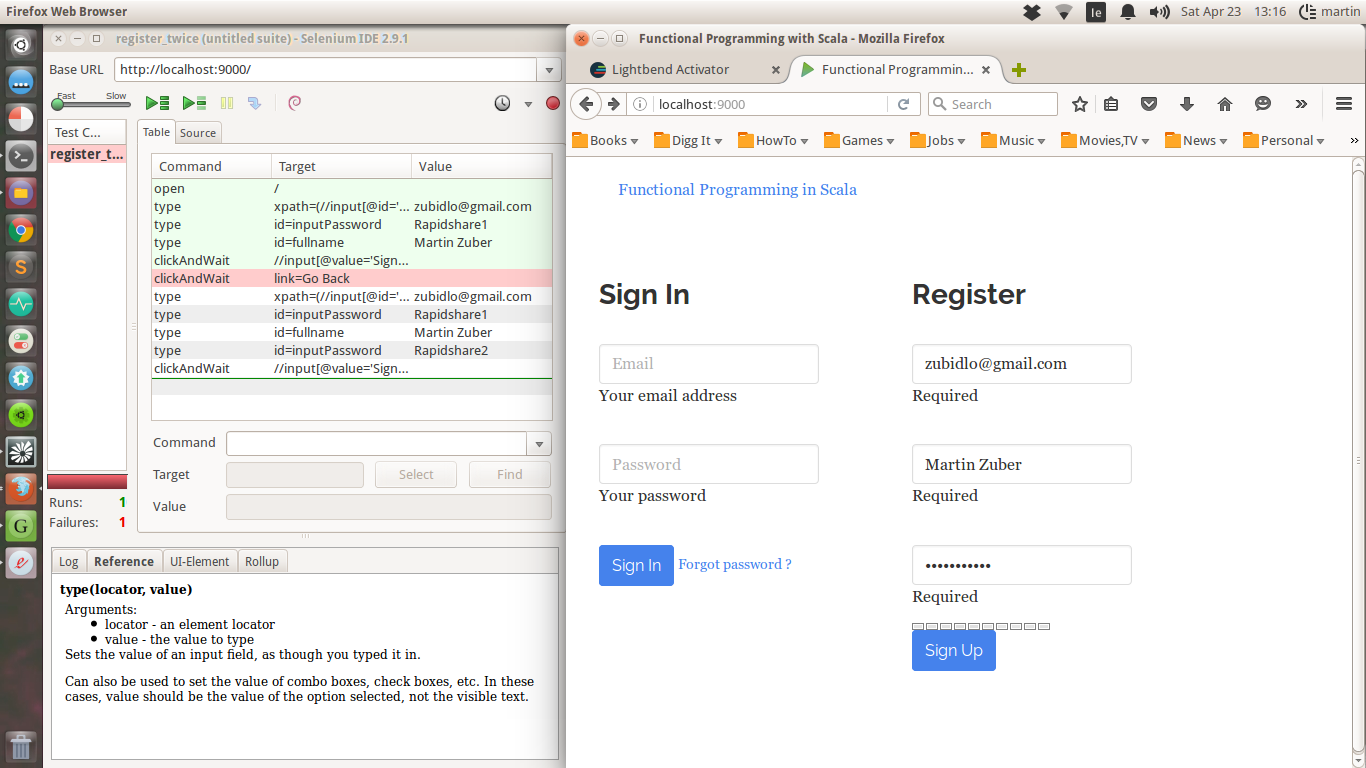
\includegraphics[width=1\textwidth, totalheight=9cm]
		{selenium_ide}
	\caption{\textit{Selenium IDE Firefox Pluggin}}
	\label{f5.3.1}
\end{figure}

All the Selenium tests are stored in the \emph{/web\_app/test/selenium\_firefox/} directory.

\subsection{Prototype 1.0}\label{5.3.1}
\subsubsection{Register Account Twice Test}\label{5.3.1.1}

User clicks register. The page will redirect to the account registered page which will inform the user that he will receive an email to confirm the registration. User clicks on \emph{"GO BACK"} button. The user is then redirected back to index page. The user then repeats the registration process with the same email supplied and clicks on the registration button.
\begin{figure}[!ht]
	\centering
		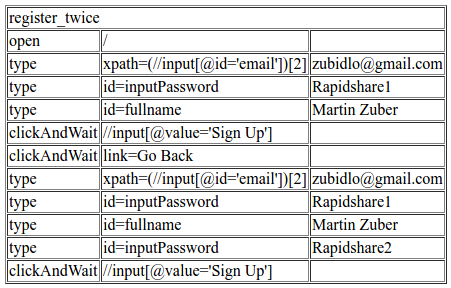
\includegraphics[width=0.6\textwidth, totalheight=5cm]
		{register_twice_test}
	\caption{\textit{Register Account Twice Actions}}
	\label{f5.3.1.1}
\end{figure}

\textbf{Bug:} The page will redirect without any explanation of just a registration form again and will not register any additional account.

\textbf{Suggested Fix:} The application should print a warning message that the account with this email address already exists and redirect to the index page.

\subsubsection{Dashboard or any of the lecture request test}\label{5.3.1.2}

\textbf{Bug:}If the dashboard page or any of the lecture pages are requested without a user login the pages are delivered which is not desired behaviour.

\textbf{Suggested Fix:} Check if dashboard checks if user email is in the session.

%____________________________section____________________________
\section{Conclusion}\label{5.4}

In the test phase I applied following test strategies:
\begin{enumerate} \item Unit tests of the models.
\item User Interface acceptance tests.
\end{enumerate}
Even though Play application supports the test of the whole application stack, I left out the testing of view rendering and controllers. The reason was that I could not make supplied test helpers work. Tutorials referring to the Play 2.2 version does not reflect the 2.5 version of the testing framework.

I found various bugs in the application, especially in the user interface which have inconsistent behaviour, not in compliance with the application specifications. After each bug fix, the regression tests were performed not the re-factored code.

In conclusion, the Play Framework has rich support for testing the web applications with some migration issues.









%_______________________________chapter_______________________________________
\chapter{Functional Programming with Scala}\label{6}

%____________________________section____________________________
\section{Introduction}\label{6.1}

As a Computer Science student at ITB, I was introduced to computer
programming through Java programming language. First, we learned the
syntax of the language. Next, we have been introduced to the
object-oriented approach to designing software and how to work with
libraries such as Swing. Later in the third year, we learned the basics
of concurrency and some design patterns for solving reoccurring
problems.

Around this time I crossed the initial steep part of the programming
learning curve and I was comfortable enough with Java to learn some
additional language features and Java Standard Edition platform
libraries. Programming with Java became my hobby and I found a time to
read additional material such as \emph{Thinking in Java} from Bruce Eckel or
\emph{Effective Java} from Joshua Bloch.

At the same time, Oracle introduced important update 8 to Java Standard
Edition platform which, among other things introduced the syntax for
anonymous functions (lambdas) and a number of libraries dedicated to
functional programming style. I was interested in this new functionality
and started to learn to implement it into my code. By playing with
\emph{lambdas}, \emph{streams}, and \emph{optionals} I got really curious about the
functional programming and wanted to learn more.

Any student who tries to learn functional programming within JVM
ecosystem will very soon become aware of \emph{Scala} programming language.
The reason is that Scala has more richer support for functional
programming than Java and hence is better suited as a vehicle for the
study.

The following material is an overview of what I learned about functional
programming in the period of 2 semesters. I uses Scala syntax to
communicate ideas with code.

%____________________________section____________________________
\section{Why Would You Read These?}\label{6.2}

\begin{lstlisting}
In the last section, I tried to articulate my interest in functional programming and my reasons for working on this project.

In this section, I will try to give you a reader some reasons to continue to read these pages.
\end{lstlisting}

In my experience, writing software is fun. For a while at least.

Before I write a software, I think about the design. I would think how to represent data and how to manipulate them. Then I start to write the code and I'm excited. It's fun. I'm transforming my ideas into a working program!

Very soon, though, I start to notice that not everything works well. I must handle exceptions, null checks and to deal with another problems not related to my design ideas. I find myself solving problems related to underlying computer and programming language.

As the software grows it starts to resemble a monster. My beautiful design is scattered around null checks, buried inside nested try-catch blocks. Every time I add something new, the program breaks in five places. Everything seems to be connected, dependent. Complexity grows exponentially and my capability to reason about the program degrades. It's just so many things to keep in mind. It is not fun any more! It's rather hard and mundane.

At that point, I'm ready to give up.

Well, in imperative programming languages, the methods are too powerful with no constraints. They can do whatever they want. They can change objects in place, write to a file, put something on a screen. They are liars too. For example, consider some `write(file)` method. She says she will write to a file. But instead she could throw 4 different exceptions. There are methods which say they do something and return a
result. But they can do something else in the process and hide that fact from the programmer.

\emph{Metaphorically it is similar to a situation when one gets a powerful car which allows him to drive anywhere. The car can drive through fields for example. One could try to reach a destination by driving straight line path. It looks like a great idea in the beginning until one ends up in a ditch with no way out.}

\subsection{Is there an alternative?}\label{6.2.1}

Functional Programming of course :-) !

Functional programming is the programming with functions, not methods. Functions are much less powerful. They follow constraints. In exchange though, they have various very useful properties which make reasoning
about them straight forward. Functions do what they say they do and never lie. They don't throw exceptions or return nulls.

Functions are associative, pluggable and composable, the same way the `Lego` blocks are. One can build a software by composing simple functions the same way as one would build a house from Lego blocks. The software complexity doesn't grow exponentially neither. Instead, a program is just a function composed of another functions. The capability to reason about the software stays constant.

Also, the solution space is smaller. One just need to learn a few ideas and how to compose them together. There are design patterns in functional programming of course, but there is not 40 of them.

\emph{It is like to have a car capable of driving on the roads only. One has much less power at the beginning, but one will safely reach the destination following the roads.}

These methaphores were quoted from \emph{Functional Programming is Terrible} talk presented by Runar Bjarnason.


%____________________________section____________________________
\section{What is Functional Programming?}\label{6.3}
\begin{lstlisting}
In the last section, I made a suggestion that there is a way to have fun while creating a software. I claimed that functional programming gives us a better way to design a software and reason about it.

In the following sections, I will discuss the functional programming definition in comparison to imperative programming paradigm.
\end{lstlisting}

\subsection{Imperative Programming Paradigm}\label{6.3.1}

Imperative programming uses statements that change the program's state. We construct programs with programming language commands and which describe how the program operates. Our programs basically tell the compiler (interpreter) how to accomplish desired results step by step.

With the addition to statements, we use subroutines call procedures or functions to modularize imperative programs. Imperative programming with procedures is called \emph{procedural programming}. Procedures have no properties or restrictions defined, for example, they may or may not take arguments and may or may not return a result value. They may modify the state of the program or crash with an error.

What imperative programs do:

\begin{enumerate}\itemsep1pt \parskip0pt \parsep0pt
\item They modify mutable variables with assignments.
\item They use control structures such as loop, break, continue, if-else statements.
\item They use procedures with no restrictions on their properties.
\end{enumerate}

\textbf{Example:}
\begin{lstlisting}[language=java]
var numbers = List(1,2,3,4,5)
var sum = 0
do {
    sum += numbers.head
    numbers = numbers.tail
  } while (numbers != Nil)

//Result:
numbers: List[Int] = List()
sum: Int = 15
\end{lstlisting}

In the example above the program calculates the sum of numbers from 1 to 5. Variables \emph{numbers} and \emph{sum} represent the mutable state which is modified in the \emph{do while loop} control structure. After the program executes the list \emph{numbers} is empty and \emph{sum} is 15.

\subsection{Functional Programming Paradigm}\label{6.3.1}

Functional programming is a programming style where the fundamental application is the application of pure functions to arguments. Functional programs are composed of functions.

What functional programs do:

\begin{enumerate}\itemsep1pt \parskip0pt \parsep0pt
\item They transform immutable values to other values.
\item They use functions and function compositions as control structures.
\item They use pure referentially transparent functions.
\end{enumerate}

\textbf{Example:}
\begin{lstlisting}[language=java]
var numbers = List(1,2,3,4,5)
  
def sumOfNumbers(numbers: List[Int]): Int = numbers match {
  case Nil => 0
  case head :: tail => head + sumOfNumbers(tail)
}
  
val sum = sumOfNumbers(numbers)

//Result:
numbers: List[Int] = List(1, 2, 3, 4, 5)
sumOfNumbers: (numbers: List[Int])Int
sum: Int = 15
\end{lstlisting}

In the example above the program calculates the sum of numbers from 1 to 5 with the usage of pure function \emph{sumOfNumbers}. This is a function which takes a \emph{List[Int]} and returns \emph{Int}. The \emph{sumOfNumbers} is defined in terms of its argument \emph{List[Int]} as follows:

\begin{itemize}\itemsep1pt \parskip0pt \parsep0pt
\item If the function receives empty list `Nil` it returns 0.
\item If the function receives a list of one or more elements it adds the first  \emph{head} to the recursive call to itself with the new list \emph{tail}.  The \emph{tail} just original list without \emph{head}. Note that \emph{head :: Nil} would match list with one.
\end{itemize}

The function application \emph{sumOfNumbers(numbers)} will in effect build following call stack:

\begin{lstlisting}[language=java]
(1 + sumOfNumbers(List(2,3,4,5))
(1 + (2 + sumOfNumbers(List(3,4,5)))
(1 + (2 + (3 + sumOfNumbers(List(4,5))))
(1 + (2 + (3 + sumOfNumbers(List(4,5))))
(1 + (2 + (3 + (4 + sumOfNumbers(List(5)))))
(1 + (2 + (3 + (4 + (5 + sumOfNumbers(Nil))))))
(1 + (2 + (3 + (4 + (5 + 0)))))
\end{lstlisting}

And when it folds it returns 15. Notice that we did not define any mutable variables anywhere in the program. Everything is immutable value \emph{val} and cannot be changed. All we do is to transform a list of numbers to its sum without changing anything.



%____________________________section____________________________
\section{Functions Everywhere}\label{6.4}
\begin{lstlisting}
In the last section, I compared the idioms of imperative and functional programming with simple examples. I stated that the building blocks of functional programs are pure functions.

In the following section, I will discuss functions and their characteristics in more detail.
\end{lstlisting}

\subsection{Pure Function}\label{6.4.1}

\begin{itemize}\itemsep1pt \parskip0pt \parsep0pt
\item The function \textbf{always} evaluates to the same result given the same argument. The word always is emphasized here. The pure function can return the same result for different arguments, but it can never return different results for the same argument.
\item Evaluation of the result does not cause any semantically observable **side effect**. Well, what are these side effects then? In Computer Science, a function or expression is said to have a side effect if it modifies some state or has an interaction with calling functions or the outside world. Basically, a function has a side effect if it does something else than returning a result. Some examples of side effects:
	\begin{enumerate}\itemsep1pt \parskip0pt \parsep0pt
	\item Modifying a variable or a data structure in place
	\item Throwing an exception or halting with an error
	\item Writing to or reading from the console or a file
	\item Drawing on the screen, updating a database, printing on a printer
	\end{enumerate}
\end{itemize}

Every function with the characteristics of a pure function is called \textbf{referentially transparent} and allow us to replace the expression in code which applies one of these functions with its result value without affecting the behaviour of the program in any way.

\textbf{Example:} Pure vs Impure
\begin{lstlisting}[language=python]
sin(x)
length(list)
random(seed)
printf(string)
\end{lstlisting}
Functions \emph{sin} and \emph{length} are pure functions because they always return the same result for the same argument and do nothing else. Function \emph{sin(0)} returns always 0 and \emph{length(List(1,2,3,4,5))} of the same list is always 5. In other words function application \emph{sin(0)} can be replaced with value 0 and function application \emph{length(List(1,2,3,4,5))} with value 5.

Functions \emph{random(seed)} and \emph{printf(string)} are impure functions because \emph{random(1)} will not always return the same result. It will return a random number from 0 to 1. Function \emph{printf(“hello world”)} will print the string literal to the console and return no result. Even that is not guaranteed. Sometimes it can throw an exception if the console is not available for example. Impure functions are called \textbf{procedures} in computer science.

\textbf{Example:} Function definition in Scala
\begin{lstlisting}[language=python]
def add(a: Int, b: Int): Int = a + b
\end{lstlisting}

The function \emph{add} is defined as a function which takes two integers and returns one integer. The \emph{add} function signature is \emph{add = (Int, Int) => Int}. We can think of functions as mappings from input to output. I this case \emph{add} is a mapping from \emph{a,b} to \emph{a + b}. We can express this fact with the following statement:

\begin{lstlisting}[language=python]
val add: (Int,Int) => Int = (a, b) => a + b
\end{lstlisting}

Because the Scala compiler supports type inference we can express the function with shorter statement:
\begin{lstlisting}[language=python]
val add = (a: Int, b: Int) => a + b
\end{lstlisting}

The compiler will \emph{infer} that \emph{add} can only return \emph{Int} value. In a specific cases we will be able to omit the arguments types as well and just write: \emph{add = (a, b) => a + b}. This form of function description is called a \emph{lambda expression}. It is basically an anonymous function, a function without name. We can read \emph{val add = (a: Int, b: Int) => a + b} as: \emph{Immutable value add is anonymous function which takes a,b and returns a + b.}

\textbf{Note:}
\begin{lstlisting}
In Scala and functional programming languages in general, functions are values. The same way the objects are values. We can assign functions to variables, pass them as arguments to other functions, create them inside the functions and return them as results of function computations. 
\end{lstlisting}

\subsection{General Terms}\label{6.4.2}

Consider a function:
\begin{lstlisting}[language=python]
val intToString: Int => String = i => i.toString
val s = intToString(123)

//Result:
intToString: Int => String = <function1>
s: String = 123
\end{lstlisting}
The immutable value \emph{intToString} is a function which takes an \emph{Int} and returns \emph{String} such as it applies \emph{toString} function to the given \emph{Int}. The immutable \emph{String} value \emph{s} is the result of \emph{intToString} function application to arguments \emph{123}.

\begin{enumerate}\itemsep1pt \parskip0pt \parsep0pt
\item The \emph{Int} and \emph{String} are \textbf{types} and represent sets of values.
\item The type \emph{Int} is a \textbf{domain} of \emph{intToString} function.
\item The type \emph{String} is a \textbf{codomain} of \emph{intToString} function.
\item The \emph{intToString} is \textbf{total function} because it is defined for every value from its domain. In other words \emph{intToString} will return a value for any possible value of type \emph{Int}
\end{enumerate}

Consider:
\begin{lstlisting}[language=python]
val stringToInt: String => Int = s => s.toInt
val i = stringToInt("123")

//Result:
stringToInt: String => Int = <function1>
i: Int = 123
\end{lstlisting}

In the contrast the \emph{stringToInt} is a \textbf{partial function} because is not defined for every value from its domain, for example application \emph{stringToInt("abc")} would crush with \emph{java.lang.NumberFormatException} exception.

\subsection{Functions as table lookups}\label{6.4.3}

As we discuss above  pure functions are mappings from domain to codomain. We can always express functions in a form of a table look up. For example, we can define \emph{stringToInt} as follows:
\begin{lstlisting}[language=python]
def stringToInt(s: String): Int = s match {
  case "1" => 1
  case "2" => 2
  case "3" => 3
  case s => ???
}
  
val i = stringToInt("1") 

//Result:
stringToInt: (s: String)Int
i: Int = 1
\end{lstlisting}

The \emph{stringToInt} is only defined for domain: \emph{{"1", "2", "3"}} and for any other value it would throw \emph{scala.NotImplementedError: an implementation is missing} error.

\textbf{Note:}
\begin{lstlisting}
Any function can be defined as a table lookup. We can think of common data structures as partial functions as well. Map ("1" => 1, "2" => 2, "3" => 3) is the same partial function as `stringToInt` and in Scala every Map inherits the PartialFunction trait. Every Scala Map is a function from its keys to its values. If fact, Many Scala data structures are partial functions.
\end{lstlisting}


%_______________________________________________________________________
\section{Higher Order Functions.}\label{6.5}
\begin{lstlisting}
In this section, I will continue to talk about functions, especially the
higher order functions.
\end{lstlisting}

\subsection{Tail Recursion and Inner Function}\label{6.5.1}

We already saw how to sum the list of numbers with a recursive function:
\begin{lstlisting}[language=python]
def sumOfNumbers(numbers: List[Int]): Int = numbers match {
  case Nil => 0
  case head :: tail => head + sumOfNumbers(tail)
}
\end{lstlisting}

And we saw how this function application will sum the numbers by building the call stack. But this function has a flow. The calls stack in Java Virtual Machine is not infinite. If we apply \emph{sumOfNumbers} to a very long list, our program will crash with \emph{java. Lang. StackOverflowError}:
\begin{lstlisting}[language=python]
var numbers = Range(1,10000).toList  
val sum = sumOfNumbers(numbers)
 
//Result:
java.lang.StackOverflowError
at scala.collection.immutable.Nil$.equals(List.scala:424)...
\end{lstlisting}

The reason for this is that recursive call is not in \textbf{tail position} meaning that when \emph{head + sumOfNumbers (tail)} is evaluated, it first applies \emph{sumOfNumbers (tail)} for each subsequent call and then adds heads. Therefore, each call stack frame must be maintained because it stores each \emph{head}. When all the recursive calls are done, only then the stack is folded and all the heads are added. There is a way around this call stack build-up by designing a recursive function differently.
\begin{lstlisting}[language=python]
def sumOfNumbers(numbers: List[Int]): BigInt = {
    def loop(accumulator: BigInt, numbers: List[Int]): BigInt = numbers match {
        case Nil => accumulator
        case head :: tail => loop(accumulator + head, tail)
    }
    loop(0, numbers)
}
  
var numbers = Range(1,10000).toList
val sum = sumOfNumbers(Range(1,10000).toList)

//Result:
sumOfNumbers: (numbers: List[Int])BigInt
numbers  : List[Int] = List(1, 2, 3...
sum: BigInt = 49995000
\end{lstlisting}

The \emph{sumOfNumbers} function application will in effect build following call stack:
\begin{lstlisting}[language=python]
(loop(0, List(1,2,3,4...))
(loop(0 + 1, List(2,3,4...))
(loop(1 + 2, List(3,4...))
(loop(3 + 3, List(4...))
...
(loop(accumulator + 10000, Nil)
\end{lstlisting}

The last call will return the \emph{accumulator} which will be already calculated as 49995000. Notice there is no stack build up and each function application differs on by its arguments. This fact can be used in the optimization technique called \textbf{tail call elimination} and a clever compiler can evaluate this kind of function application with just a one stack frame. Scala supports this type of optimizations. You can even mark your recursive function with \emph{@tailrec} annotation and the function will not compile until is not tail recursive.

\textbf{Note:}
\begin{lstlisting}
The point of this exercise was to demonstrate that loop function is defined inside sumOfNumbers function. This is common practice in functional programming languages. Functions are first class values and to define an inner function is nothing stranger than to define a new variable inside a function.
\end{lstlisting}

\subsection{Functions as arguments}\label{6.5.2}

The higher order function is defined as any function which:
\begin{enumerate}\itemsep1pt \parskip0pt \parsep0pt
\item takes one or more functions as arguments
\item returns a function as its result
\end{enumerate}

The simplest possible example of a function which takes a function as an argument would be:
\begin{lstlisting}[language=python]
def apply(a: Int, function: Int => Int): Int = function(a)
val result = apply(5, a => a * a)

//Result:
apply: (a: Int, function: Int => Int)Int
result: Int = 25
\end{lstlisting}
The \emph{apply} function \emph{(Int, Int => Int) => Int} takes an \emph{Int} and function \emph{Int => Int} and returns an \emph{Int}. In our case the function just applies the \emph{Int} argument to \emph{Int => Int} function. Think of it as a delegation. Give me an integer and a function which takes an integer and I will apply that integer to given function.
With \emph{apply(5, a => a * a)} we applied 5 to the anonymous function \emph{a => a * a} which just multiplies the argument \emph{a} by itself.

\subsection{Functions as results}\label{6.5.3}

Let's define function \emph{adder}:
\begin{lstlisting}[language=python]
def adder(a: Int): Int => Int = b => b + a
val addOne = adder(1)
val addFive = adder(5)

val eleven = addOne(10) + addFive(10)

//Result:
adder: (a: Int)Int => Int
addOne: Int => Int = <function1>
addFive: Int => Int = <function1>
eleven: Int = 26
\end{lstlisting}

\begin{enumerate}\itemsep1pt \parskip0pt \parsep0pt
\item \emph{adder} is a function \emph{Int => (Int => Int)} which takes an \emph{Int} and returns a function \emph{Int => Int}
\item \emph{addOne} is a function \emph{Int => Int} which takes \emph{adder} function applied to 1 and returns a function \emph{b => b + 1}
\item \emph{addFive} is a function \emph{Int => Int} which takes \emph{adder} function applied to 5 and returns a function \emph{b => b + 5}
\item \emph{eleven} is the result value of \emph{addOne(10) + addFive(10)} and equals 11 + 15, hence 26
\end{enumerate}

\textbf{Note:}
\begin{lstlisting}
The higher order function is a very powerful concept, which allows us to construct elegant programs using function compositions. There are whole libraries of predefined higher order functions in every functional programming language. For example Clojure programming language comes with around 500 predefined functions in its core library. Scala comes with rich interfaces full of useful higher order functions as well. I will show some examples of functions defined on sequences in the next section.
\end{lstlisting}









%_______________________________chapter_______________________________________
\chapter{Conclusion and Further Work}\label{7}

%____________________________section____________________________
\section{Introduction}\label{7.1}
//TODO

%____________________________section____________________________
\section{Achievements}\label{7.2}
//TODO

%____________________________section____________________________
\section{Personal Gain}\label{7.3}
//TODO

%____________________________section____________________________
\section{Further Work}\label{7.4}
//TODO

%____________________________section____________________________
\section{Conclusion}\label{7.5}
//TODO

%_______________________________Bibliography_______________________________________
\addcontentsline{toc}{section}{Bibliography}
\bibliographystyle{plain}
\setstretch{1}
\begin{thebibliography}{99}

\bibitem{1}
Neil Ford,
\emph{Functional thinking: Why functional programming is on the rise},
\url{http://www.ibm.com/developerworks/library/j-ft20/},
(2013-01-25)

\bibitem{2}
Typesafe,
\emph{Scala, Object-Oriented Meets Functional},
\url{http://www.scala-lang.org/},
(2002-2015)
	
\bibitem{3}
Typesafe,
\emph{Scala in the Enterprise},
\url{http://www.scala-lang.org/old/node/1658},
(2012-01-19)

\bibitem{4}
Brikman, Yevgeniy,
\emph{The Play Framework at LinkedIn: Productivity and Performance at Scale},\\
\url{https://www.youtube.com/watch?v=8z3h4Uv9YbE&ab_channel=NewCircleTraining},
(2013-06-26)

\bibitem{5}
Wampler, Dean,
\emph{We Won! How Scala Conquered the Big Data World.},
\url{https://www.youtube.com/watch?v=AHB6aJyhDSQ&ab_channel=NewCircleTraining},
(2015-03-01)

\bibitem{6}
theotown,
\emph{Akka wins 2015 JAX Award for Most Innovative Open Source Technology},
\url{https://www.typesafe.com/blog/akka-wins-2015-jax-award-for-most-innovative-open-technology},
(2015-03-23)
	
\bibitem{7}
Wikipedia,
\emph{Free software programmed in Scala},
\url{https://en.wikipedia.org/wiki/Category:Free_software_programmed_in_Scala},
(2015-01-05)
	
\bibitem{8}
Wikipedia,
\emph{Play Framework},
\url{https://en.wikipedia.org/wiki/Play_framework},
(2015-10-04)
	
\bibitem{9}
Paul Chiusano, Runar Bjarnason,
\emph{Functional Programming in Scala.},
Shelter Island, NY 11964,
Manning Publications Co., 2015. ISBN 9781617290657.

\bibitem{10}
Dean Wampler, Alex Payne,
\emph{Programming Scala, Second Edition.},
1005 Gravenstein Highway North, Sebastopol, CA 95472,
O’Reilly Media, Inc., 2015. ISBN: 978-1-491-94985-6.
	
\bibitem{11}
Peter Hilton, Erik Bakker, Francisco Canedo,
\emph{Play For Scala.},
Shelter Island, NY 11964,
Manning Publications Co., 2014. ISBN 9781617290794.

\bibitem{12}
Hudak, P.,
\emph{The Conception, Evolution, and Application of Functional Programming Languages.},
s.l.:Yale University Department of Computer Science,
1989

\bibitem{13}
Hristakeva, M., Vuppala, R.,
\emph{A Survey of Object Oriented Programming Languages.},
Santa Cruz: Univ. of California.
2009

\bibitem{14}
Hughes, J.,
\emph{Why Functional Programming Matters.},
Goteborg Institutionen for Datavetenskap,
Chalmers Tekniska Hogskola, 1984


\bibitem{15}
Goyri, A., Franklin, L., Dig, D., Lahoda, J.,
\emph{Crossing the Gap from Imperative to Functional, Programming through Refactoring.},
Saint Petersburg: s.n.,
2013

\bibitem{16}
Roy, P. V.,
\emph{Programming Paradigms for Dummies: What Every Programmer Should Know.},
s.l.:IRCAM/Delatour,
2009

\bibitem{17}
Odersky M., Altherr P., Cremet V., Dragos I., Dubochet G.,
\emph{An Overview of the Scala Programming Language},
s.l.:IRCAM/Delatour,
Second Edition,
2006

\bibitem{18}
Wikipedia,
\emph{Read-Eval-Print Loop},
\url{https://en.wikipedia.org/wiki/Read-eval-print_loop},
(2015-11-21)

\bibitem{19}
Netty is an asynchronous event-driven network application framework ...,
\emph{Netty Project},
\url{http://netty.io/},
2016

\bibitem{20}
Markdown,
\emph{Daring Fireball},
\url{https://daringfireball.net/projects/markdown/	},
2002-2016

\bibitem{21}
Ubuntu 14.04.3 LTS,
\emph{Canonical Ltd.},
\url{http://www.ubuntu.com/download/desktop}
2016

\bibitem{22}
Gummi, The Simple LaTeX editor,
\emph{alexandervdm},
\url{https://github.com/alexandervdm/gummi},
2016

\bibitem{23}
Remarkable,
\emph{Jamie McGowan},
\url{http://remarkableapp.github.io/},
2015

\bibitem{24}
Intellij IDEA,
\emph{JetBrains s.r.o},
\url{https://www.jetbrains.com/idea/},
2000-2016

\bibitem{25}
Git,
\emph{Linus Torvalds, Software Freedom Conservancy},
\url{https://git-scm.com/},
2005-2016

\bibitem{26}
Heroku Play Framework Support,
\emph{Heroku.com},
\url{https://devcenter.heroku.com/articles/play-support},
2016-01-22

\bibitem{27}
Deploying Play Framework Apps with the Azure Toolkit for Eclipse,
\emph{Kirk Evans[MSFT]},
\url{https://blogs.msdn.microsoft.com/kaevans/2015/05/12/deploying-play-framework-apps-with-the-azure-toolkit-for-eclipse/},
2015-05-12

\bibitem{28}
The High Velocity Web Framework For Java and Scala,
\emph{Typesafe},
\url{https://www.playframework.com},
2016

\bibitem{29}
The Interactive Build Tool,
\emph{Typesafe},
\url{http://www.scala-sbt.org/},
2015

\bibitem{30}
Play Framework,
\emph{Scala Twirl Engine},
\url{https://github.com/playframework/twirl},
2016

\bibitem{31}
Avaje,
\emph{Ebean ORM for Java/Kotlin},
\url{http://ebean-orm.github.io/},
2016

\bibitem{32}
LightBend Inc,
\emph{LightBend Reactive Platform},
\url{https://www.lightbend.com/products/lightbend-reactive-platform},
2016

\bibitem{33}
Lightbend Inc,
\emph{Akka},
\url{http://akka.io},
2016

\bibitem{34}
W. Richard Stevens, Stephen A. Rago
\emph{Advanced Programming in the UNIX Environment, Third Edition},
Addison-Wesley
2013 May, ISBN-13: 978-0-321-63773-4

\bibitem{35}
mindrot.org,
\emph{jBCrypt},
\url{http://www.mindrot.org/projects/jBCrypt/},
2016-01-30

\end{thebibliography}
\end{document}